
\chapter{Motivation, Theory, Critical Analysis, \& Novelty} \label{ch:theory}

\section{\hlc[cyan]{Chapter Purpose \& Structure}}

This chapter aims to advance Research Question 1: 

\blockquote{ 1. What aspects of systems architecture (and systems engineering in general) are relevant and useful for approaching issues of sustainability in complex \acf{sets}? In particular, how can they be adapted using techniques from collaborative planning theory and other critical approaches to enable avoid the technocratic excesses of the past?}

It accomplishes this by supplying Research Deliverable 1a: ``A critical analysis of systems engineering, \acf{gis}, and the other fields relied upon in this work." This chapter thus serves both as a survey of the relevant literature to the construction of the \acf{evdt} framework (which is itself laid out in Chapter \ref{ch:evdt}) and as a critical analysis of some of that literature.

The first portion of this chapter, Section \ref{sec:motivation}, seeks to expand upon the research problems and questions laid out in Section \ref{sec:questions}. It lays out the motivation and theoretical underpinnings of this work. It can thus be understood as an attempted answer of the simultaneously singular and multifaceted question: ``Why?" Specific topics are organized in order of application domain (sustainable development) $\rightarrow$ methodological fields grounded in engineering and the natural sciences (systems engineering and remote observation) $\rightarrow$ methodological fields grounded in planning, development, and activism (collaborative development, scenario planning, and \acfp{dss}). \ac{gis} is situated between the latter two categories. Obviously this is a somewhat reductionist categorization (has indicated by the hybrid positioning of \ac{gis} and these fields have significantly influenced each other over the course of the past century. These fields were chosen to shore up one another's defects and to amplify each other's strong points. The pressing need for sustainable development. The systems thinking and design tools of systems engineering. The diversity of data from remote observation. The interest in human society and problems from collaborative planning and development. A desire to support decisions rather than make them for other communities.

The second portion of the chapter, Section \ref{sec:critiques}, turns towards to critiques of the literature and the concept of this thesis. It is an attempt to recognize and preemptively address potential pitfalls of the approach taken in this thesis. These are primarily fundamental or ethical concerns, as opposed to mere questions of implementation, the latter of which are largely held for Chapter \ref{ch:discussion}. The connections between the particular fields to the particular critiques are shown in Figure \ref{fig:lit_survey_structure} below.

The final portion of the chapter, Section \ref{sec:chap2-conc}, summarizes the lessons and findings of the literature survey and critiques that will be relevant to the development of the \ac{evdt} Framework in Chapter \ref{ch:evdt}.

\begin{landscape}
\begin{figure}[t]
	\centering
	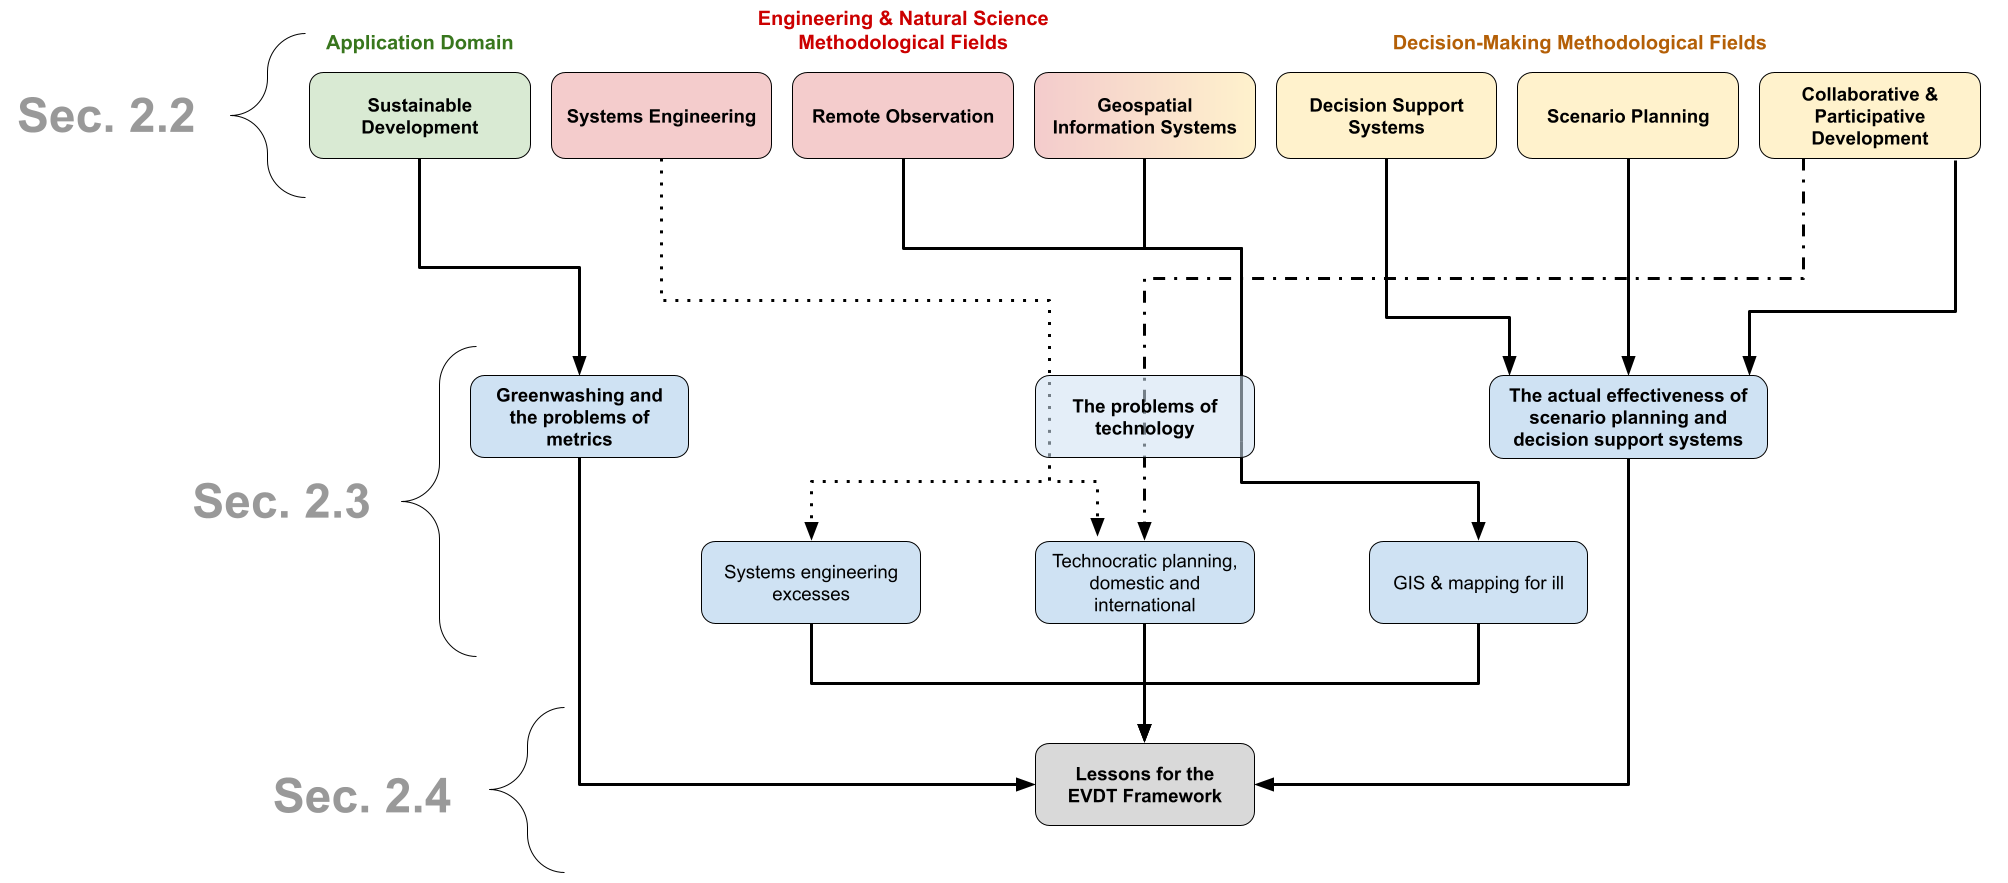
\includegraphics[scale=0.3]{Figures/chap2/lit_survey_structure.png}
	\caption[Structure of Chapter 2]{Structure of Chapter 2}
	\label{fig:lit_survey_structure}
\end{figure}
\end{landscape}

\section{\hlc[green]{Motivation \& Literature Survey}} \label{sec:motivation}

The question of motivation includes several elements. Why sustainable development? Why remote observation data? Why systems architecture and engineering? Why these particular case studies? Why me? This section will address these questions as well as lay the groundwork for the discussion of several critiques of the chosen approach that takes place in Section \ref{sec:critiques}.

\subsection{\hlc[green]{Personal Motivation}}

My background may make my interest in this work, collaborative modeling for sustainable development, seem a bit odd. Almost all of my prior work was either funded by the military or done directly for the military, from improving weapons testing procedures at Sandia National Labs to defense acquisition policy analysis for my masters degree at \ac{mit} to summers spent at the RAND Corporation helping the US military to plan aircraft and air defense acquisitions, to name just a few. My one purely private sector job (an engineering internship at a fossil fuel refinery on the coast of Texas) was hardly emblematic of a great commitment to sustainability.

In another way, however, I am merely following in a well trod, if problematic, pathway. Like Jennifer Light \cite{lightWarfareWelfareDefense2005}, I was exposed to scenario planning and other forms of decision support tools during summers working at the RAND Corporation. And like numerous \ac{mit} scholars (Jay Forrester, Norbert Wiener, Joseph Weizenbaum, the list goes on) I have pivoted from, or perhaps built upon, my experience with military engineering to instead tackle societal development problems. The convergence of this two institutions is not something to be passed over. "Support for applying cybernetic principles to research on nonliving systems emerged from organizations... studying management, engineering and control. RAND and \ac{mit} stood at the forefront of this trend. With their heritage of mathematical innovation and ties to the armed forces... these and cognate institutions offered ideal laboratories to transform cybernetic principles into management practices." \cite{lightWarfareWelfareDefense2005} 

There is a key difference between me and my predecessors (or so I would like to believe). While some of these  (Weizenbaum in particular \cite{lightWarfareWelfareDefense2005}) came to have doubts about the consequences of applying military-originated technical methods to civilian applications, most of them did not. They resolutely swept aside complications, objections, and planning professionals to solve the problems that they identified in their own way. They built names and careers in this way, but also caused significant harms in their hubris, as I will discuss more later in this chapter.

My background and perspective is somewhat different from them in certain ways, however. My undergraduate mechanical engineering degree was obtained alongside a philosophy degree. My masters aerospace engineering degree was obtained alongside a technology policy degree. And now, over the course of my doctorate, I have invested time in taking development and planning classes, reading foundational texts, and engaging with my antiracist and anticolonialist peers in Space Enabled. My education in matters of urban development and ethics is thus more significant than the one-month seminars that \ac{mit} and the University of California provided to aerospace workers in 1971 to prepare them for local government positions \cite{lightWarfareWelfareDefense2005}. 

Finally, I have the history, both positive and negative, of my \ac{mit} predecessors to inform my actions, in a way that they did not. For these reasons, I often find myself more sympathetic to the contemporary critics of some of these \ac{mit} scholars, such as Ida Hoos \cite{hoosSystemsAnalysisPublic1983}. This, of course, raises the question of why then am I proceeding with this work anyways.	

The answer to that is multifaceted. For one, I believe that the relevant fields have advanced significantly and, to some extent at least, have learned from their prior missteps. This is elaborated on in my detail throughout this chapter. Another aspect is that I (and my advisor evidently) believe that my knowledge and systems engineering in general does still have something to offer humanity beyond building rockets. Additionally, I and my peers, with our particular commitment to the principles outlined earlier, may have an important role to play on influencing the aerospace/systems engineering communities, urging them to curb their worst impulses and learn from their own history. Finally, it is because I want to be of service to humanity. As my aerospace education and career progressed, I found myself increasingly faced with only two options: "pure" scientific work or defense work. Reluctant to choose either, I was being quickly sucked into the gravity of the default: the aerospace defense sector. The Space Enabled Research Group, and the work detailed in this thesis in particular, offered me a third option, to apply my skills and interests to directly help humans on Earth. Now all that is left to is to do it.

\subsection{\hlc[green]{Why Sustainable Development?}} \label{sec:sustainable_development}

Before exploring the various methodologies and theoretical frameworks used in this work, it is worth exploring exactly what it is we are hoping to accomplish and why it is important. We need to talk about sustainable development.
 
\subsubsection{\hlc[green]{What is Sustainable Development?}} \label{sec:sustain}

The term \textit{sustainable development} is simultaneously one that invites immediate, intuitive understanding, and yet can remain frustratingly vague. \textit{Sustainable} here means something somewhat more specific than its general definitions of "able to be maintained or kept going" or "capable of being supported or upheld." Instead, it builds upon these and gains some association with the natural environment: "pertaining to a system that maintains its own viability by using techniques that allow for continual reuse" \cite{DefinitionSustainableDictionary}. As to what "system" we are talking about here, the "development" half of sustainable development, we mean generally, human society and wellbeing. This is of course still much too vague, so let us turn to the first official use of the term, which was in the 1987 report by the \ac{un} World Commission on Environment and Development, commonly known as the Brundtland Report, after the name of the chair of the commission. This report defined sustainable development as "the development that meets the needs of the present without compromising the ability of future generations to meet their own needs" \cite{worldcommissiononenvironmentanddevelopmentOurCommonFuture}. We have now helpfully clarified the time scale under which this system needs to "maintain its own viability" but still have done little to clarify what aspects of human society are included within "development." 

In 1992, the \ac{un} provided more detail in the Rio Declaration on Environment and Development. In this report, they said that "human beings are at the centre of concerns for sustainable development. They are entitled to healthy and productive life in harmony with nature." Furthermore, they state that eradicating poverty is "an indispensable requirement for sustainable development" and environmental protection constitutes "an integral part of the development process" \cite{unitednationsconferenceonenvironmentanddevelopmentRioDeclarationEnvironment1992}. So we know have several key components, including human health and productivity, the protection of the natural environment, and the elimination of poverty. It is still unclear whether this is a complete list, however, and, if so, what are the connections between these components.

Official clarification would come in 2002, at the UN World Summit on Sustainable Development in Johannesburg. There we get the following \cite{worldsummitonsustainabledevelopmentPlanImplementationWorld2002}:

\blockquote{These efforts will also promote the integration of the three components of sustainable development — economic development, social development and environmental protection — as interdependent and mutually reinforcing pillars. Poverty eradication, changing unsustainable patterns of production and
consumption, and protecting and managing the natural resource base of economic and social development are overarching objectives of and essential requirements for sustainable development.}

We now have three linked components along with a set of potential actions for implementation. This is the definition that would stick and become commonplace. From this has been built research fields and massive multi-governmental interventions. Jeffery Sachs describes this further, "As an intellectual pursuit, sustainable development tries to make sense of the interactions of three complex systems: the world economy, the global society, and the Earth's physical environment... Sustainable development is also a normative outlook of the world, meaning that it recommends a set of goals to which the world should aspire... SDGs call for socially inclusive and environmentally sustainable growth." \cite{sachsAgeSustainableDevelopment2015}

Questions remain, however. Why all this effort? And what are these SDGs?

\subsubsection{\hlc[green]{Why is Sustainable Development Important?}}

As former \ac{un} Secretary-General Ban Ki-moon put it:"Sustainable development is the central challenge of our times" \cite{sachsAgeSustainableDevelopment2015}. Despite significant progress in certain domains and certain regions, many individuals and communities are still suffering from severe privations of food, water, healthcare, and more. This is no mere issue of production, but is also connected with issues of allocation (economic inequality is swiftly rising in many parts of the world, including in the author's own country), political mismanagement and oppression, and environmental changes. This work will not detail these numerous concerns (instead I recommend Jeffrey Sach's \textit{The Age of Sustainable Development} for an accessible survey), but it is worth point out that the last of these issues, that of environmental changes, is particularly important as it shapes how we can seek to rectify the others. Historical means of economic development (such as the extensive use of fossil fuels) is no longer seen as sustainable, due to humanity butting up against and even exceeding certain planetary boundaries or capacity limits, particularly those of climate change, biodiversity loss, ocean acidification, and the nitrogen cycle, as seen in Figure \ref{fig:boundaries}.

\begin{figure}[h]
	\centering
	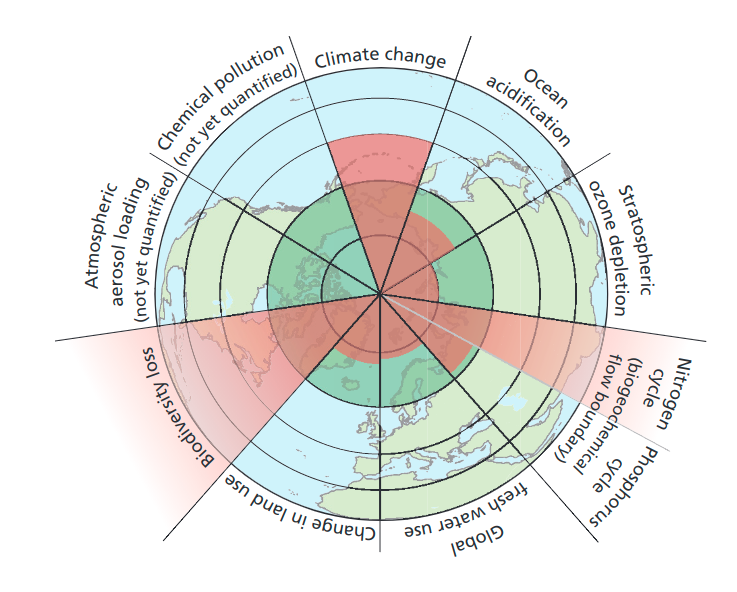
\includegraphics[scale=0.4]{Figures/chap2/Planetary_Boundaries.png}
	\caption[Planetary Boundaries]{Planetary Boundaries. From \cite{rockstromSafeOperatingSpace2009}}
	\label{fig:boundaries}
\end{figure}

While the impacts of these excesses will be felt globally, they will most heavily fall upon some of the poorer and historically oppressed states, harming those with the least capacity of absorb such impacts and thereby potentially exacerbating global inequality. The spatial variation of the estimated impacts of climate change, for instance, can be seen in Figure \ref{fig:vulnerability}.

\begin{figure}[h]
	\centering
	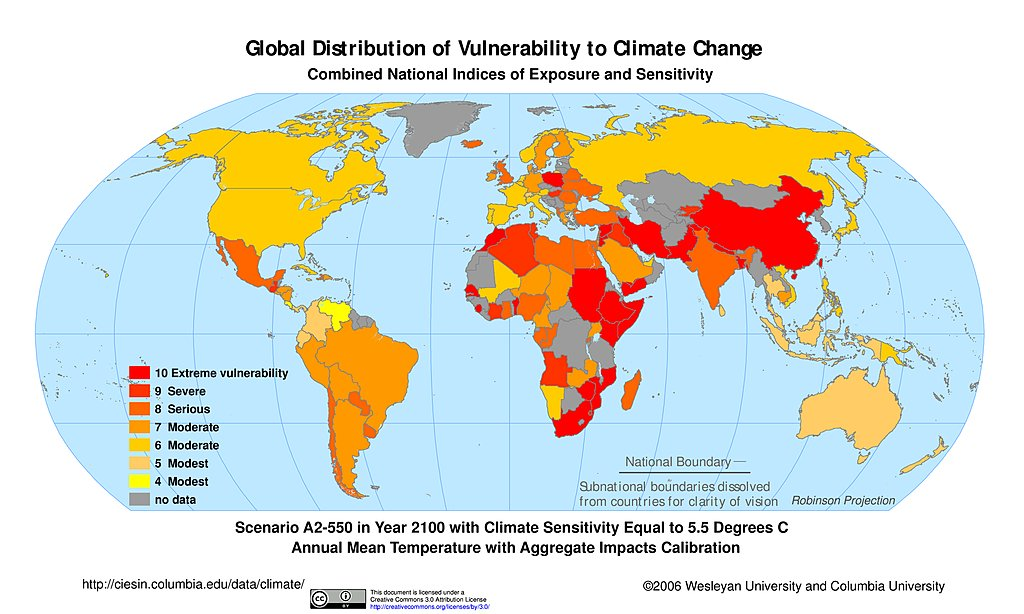
\includegraphics[scale=1.7]{Figures/chap2/vulnerability_map.jpg}
	\caption[Assessment of global distribution of vulnerability to climate change]{Assessment of global distribution of vulnerability to climate change. From \cite{yoheSyntheticAssessmentGlobal2006}}
	\label{fig:vulnerability}
\end{figure}

Furthermore, as was suggested by the Johannesburg definition of sustainable development, the effects of violating these planetary boundaries will not be limited to a particular domain of human life. Table \ref{table:bau} estimates such multi-domain impacts on different regions of the world if major, international corrective efforts are not undertaken immediately. The numerous connections between these domains is a key motivation for this work and for the methods chosen, as will be seen later.

\begin{table}[H]
\begin{minipage}{\textwidth}
\caption[Estimated impacts of "business-as-usual" by domain and region.]{Estimated impacts of "business-as-usual" by domain and region. H=High; M=Moderate. Adapted from \cite{rockstromSustainableDevelopmentPlanetary2013} and \cite{sachsAgeSustainableDevelopment2015} \protect\footnotemark[1]}
\label{table:bau}
\begin{center}
\tiny
\begin{tabular}{ | L{2cm} | C{1cm} | C{1cm} | C{1cm} | C{1cm} | C{1cm} | C{1cm} | C{1cm} | C{1cm} | } \hline
& North America & Latin America \& Caribbean & Europe & Middle East \& North Africa & Sub-Saharan Africa & South \& Central Asia & Southeast Asia \& Pacific & East Asia \\ \hline

Food Insecurity \& Malnutrition & & & & \cellcolor{red!25} H & \cellcolor{red!25} H & \cellcolor{red!25} H & \cellcolor{yellow!25} M  & \cellcolor{yellow!25} M \\ \hline

Poverty & & & & \cellcolor{yellow!25} M & \cellcolor{red!25} H & \cellcolor{red!25} H & \cellcolor{yellow!25} M  & \cellcolor{yellow!25} M  \\ \hline

Land Use Change & & \cellcolor{red!25} H & & & \cellcolor{red!25} H & \cellcolor{yellow!25} M  & \cellcolor{yellow!25} M  & \cellcolor{yellow!25} M  \\ \hline

Soil Degradation & & & & \cellcolor{yellow!25} M  & \cellcolor{red!25} H & \cellcolor{red!25} H   & \cellcolor{yellow!25} M  & \cellcolor{red!25} H   \\ \hline

Water Shortage & \cellcolor{yellow!25} M & & & \cellcolor{red!25} H & \cellcolor{red!25} H & \cellcolor{red!25} H & \cellcolor{yellow!25} M  & \cellcolor{yellow!25} M \\ \hline

Water \& Air Pollution & \cellcolor{yellow!25} M & & \cellcolor{yellow!25} M & \cellcolor{yellow!25} M  & &\cellcolor{red!25} H  & \cellcolor{red!25} H  & \cellcolor{red!25} H \\ \hline

Biodiversity Loss & \cellcolor{yellow!25}  & \cellcolor{red!25} H  & \cellcolor{yellow!25} M & \cellcolor{yellow!25} M  & \cellcolor{yellow!25} M & \cellcolor{yellow!25} M  & \cellcolor{red!25} H  & \cellcolor{red!25} H \\ \hline

Sea Level Rise & \cellcolor{yellow!25} M & \cellcolor{yellow!25} M & \cellcolor{red!25} H & \cellcolor{yellow!25} M & \cellcolor{red!25} H & \cellcolor{red!25} H &\cellcolor{red!25} H  & \cellcolor{red!25} H \\ \hline

Ocean Acidification &  \cellcolor{yellow!25} M & \cellcolor{red!25} H & \cellcolor{red!25} H & \cellcolor{yellow!25} M & \cellcolor{yellow!25} M  & \cellcolor{yellow!25} M & \cellcolor{red!25} H & \cellcolor{yellow!25} M \\ \hline
\end{tabular}
\end{center}
\end{minipage}
\end{table}

\footnotetext[1]{It should be noted that, despite the latter of these two sources citing the former, the two sources differ in noticeable ways, with no explanation provided in either document. Where they are in conflict, I have chosen to use the latter source. In the former source, there is also a error: Ocean Acidification in the Middle East / North Africa is listed as "H" but the cell is in yellow. The correct entry is not known, so I have gone with "M" in yellow here in order to avoid overstatement.}

A key reason why these planetary boundaries have been so recklessly exceeded despite the enormous human costs that will result is that these aspects of the environment have historically been both undervalued and poorly understood (at least by those championing economic development). Historically, surveys and quantifications of the natural environment focused primarily, or even entirely, on resources that could be extracted and exploited for economic benefit. In early forest surveys, for instance, "Missing... were all those parts of trees, even revenue-bearing trees, which might have been useful to the population but whose value could not be converted into fiscal receipts" \cite{scottSeeingStateHow2020}. Just as these factors were missing from accountings of the natural environment, so were they missing form accounts of human society. "Non-human animals are rarely considered within the realms of social theory, and yet... animals can be regarded as a `marginal social group' that is `subjected to all manner of socio-spatial inclusions and exclusions.'" (\cite{philolAnimalsGeographyCity1995,westcoatBringingAnimalsBack1995,wolchAnimalGeographiesPlace1998}as paraphrased in \cite{harrisRethinkingMapsMorethanhuman2011}). While these authors were referring primarily to animals, it is also  I would argue that this includes plants too, as is particularly evident in the common definition of a weed as a plant growing where it is not wanted.

Fortunately, economists and earth scientists in recent decades have embarked on an effort to better understand and catalog such \textit{ecosystem services}, that is to say, the various benefits that humans are provided by the natural environment and healthy ecosystems in particular. Figure \ref{fig:services_wellbeing} illustrates these connections between the environment and human wellbeing, along with the degree to which these connections are mediated by socioeconomic factors. While this kind of accounting can easily veer into a "commodification of nature", the concept of ecosystem services has proven to be a valuable method for analysis trade-offs in environmental and environmental-adjacent policy \cite{mccauleySellingOutNature2006, guoEconomicsClimateChange2021}. This work has progressed to the extent that there is now a regularly updated database of almost 5,000 value observations of ecosystem services in a wide variety of regions and biomes \cite{grootEcosystemServicesValuation2020}. Cataloging such ecosystem services is only one step, however. We must also present this data in useful ways to decision-makers  so that they may act upon it, as well has provide them with the tools for them to identify additional, uncataloged ecosystem services in their own communities.

\begin{figure}[h]
	\centering
	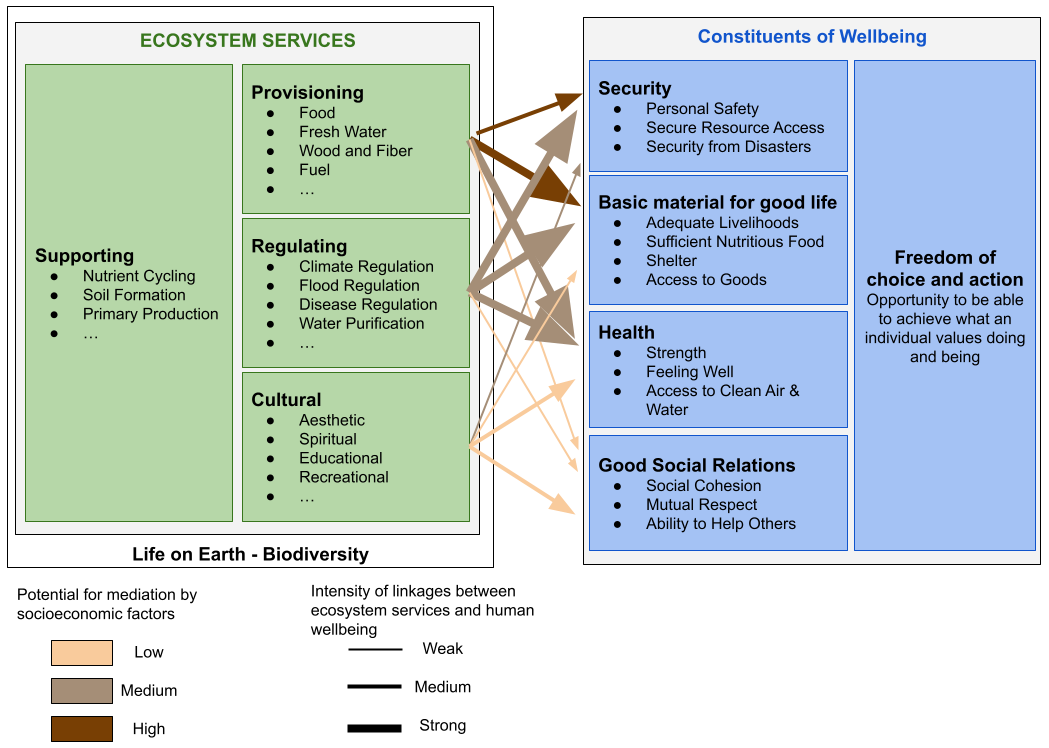
\includegraphics[scale=0.35]{Figures/chap2/services_wellbeing.png}
	\caption[Linkages between categories of ecosystem services and components of human wellbeing]{Linkages between categories of ecosystem services and components of human wellbeing. Adapted from \cite{reidEcosystemsHumanWellbeing2005}}
	\label{fig:services_wellbeing}
\end{figure}

It is important to note that common to all these perspectives on sustainable development is the interaction of multiple domains that have historically been considered separately. In this way, the pursuit of sustainable development can considered to be a combination of the established fields of \acf{sts} \cite{rouseUnderstandingChangeComplex2012,siddiqiSociotechnicalSystemsSustainability2017,sussmanTeachingComplexSociotechnical2010} and \acf{ses} \cite{elsawahEightGrandChallenges2020}, thereby making sustainable development contexts into \acf{sets}.

\subsubsection{\hlc[green]{What about the Sustainable Development Goals?}}

At the end of Section \ref{sec:sustain}, I quoted a passage that referred to the \acp{sdg}, though I did not explain what these were. Now I shall address that deficiency, as the \acp{sdg} are a key part of how sustainable development is currently thought about around the world, to the extent that Sachs wrote that, "Our new era will son be described by new global goals, the SDGs" \cite{sachsAgeSustainableDevelopment2015}. In order to understand the \acp{sdg}, however, we must first go back fifteen years prior to their creation, when the nations of the world sought to proactively face the new millennium. In 2000, the \ac{un} established eight \acp{mdg} that the nations of the world pledged to pursue for the next fifteen years. These were [emphasis added]:

\begin{enumerate} \setlength{\itemsep}{0pt} \setlength{\parskip}{0pt}
	\item To eradicate extreme poverty and hunger
	\item To achieve universal primary education
	\item To promote gender equality and empower women
	\item To reduce child mortality
	\item To improve maternal health
	\item To combat HIV/AIDS, malaria, and other diseases
	\item To ensure environmental \textbf{sustainability}
	\item To develop a global partnership for development
\end{enumerate}
    

Within each of these goals were various more specific \textit{targets}, each with a set of quantitative metrics or \textit{indicators}. While significant progress towards the \acp{mdg} was made over the course of those fifteen years, significant issues persisted after their conclusion \cite{inter-agencyandexpertgrouponmdgindicatorsMillenniumDevelopmentGoals2015}. By the year 2015, numerous changes had occurred. There was an increased interest in recognizing the interdependence of the challenges facing humanity, treating causes rather than symptoms, and in collective action rather than donor-driven action. The \acp{mdg}, for instance, often focused exclusively on developing countries and what developed countries could offer them, sometimes explicitly so, such as in Target 8.E: "In cooperation with pharmaceutical companies, provide access to affordable essential drugs in developing countries." 

By the year 2015, there was an heightened recognition of disparities and issues within all nations, not just the developing ones. These factors, coupled with the rise in public salience regarding sustainability, resulted in the successors to the \acp{mdg}, the \acp{sdg}. The \acp{sdg} were set in 2015 and are intended to serve as global goals for the international community until 2030. It expanded the number of goals from 8 to 17, each with its own set of indicators and targets \cite{unitednationsTransformingOurWorld2015}. Some of the original \acp{mdg} were split into multiple, more specific goals (e.g. \#1 became \#2 and \#3) while other \acp{sdg} are wholly novel. The abbreviated forms of these new goals can be seen in Figure \ref{fig:sdgs}.

\begin{figure}[h]
	\centering
	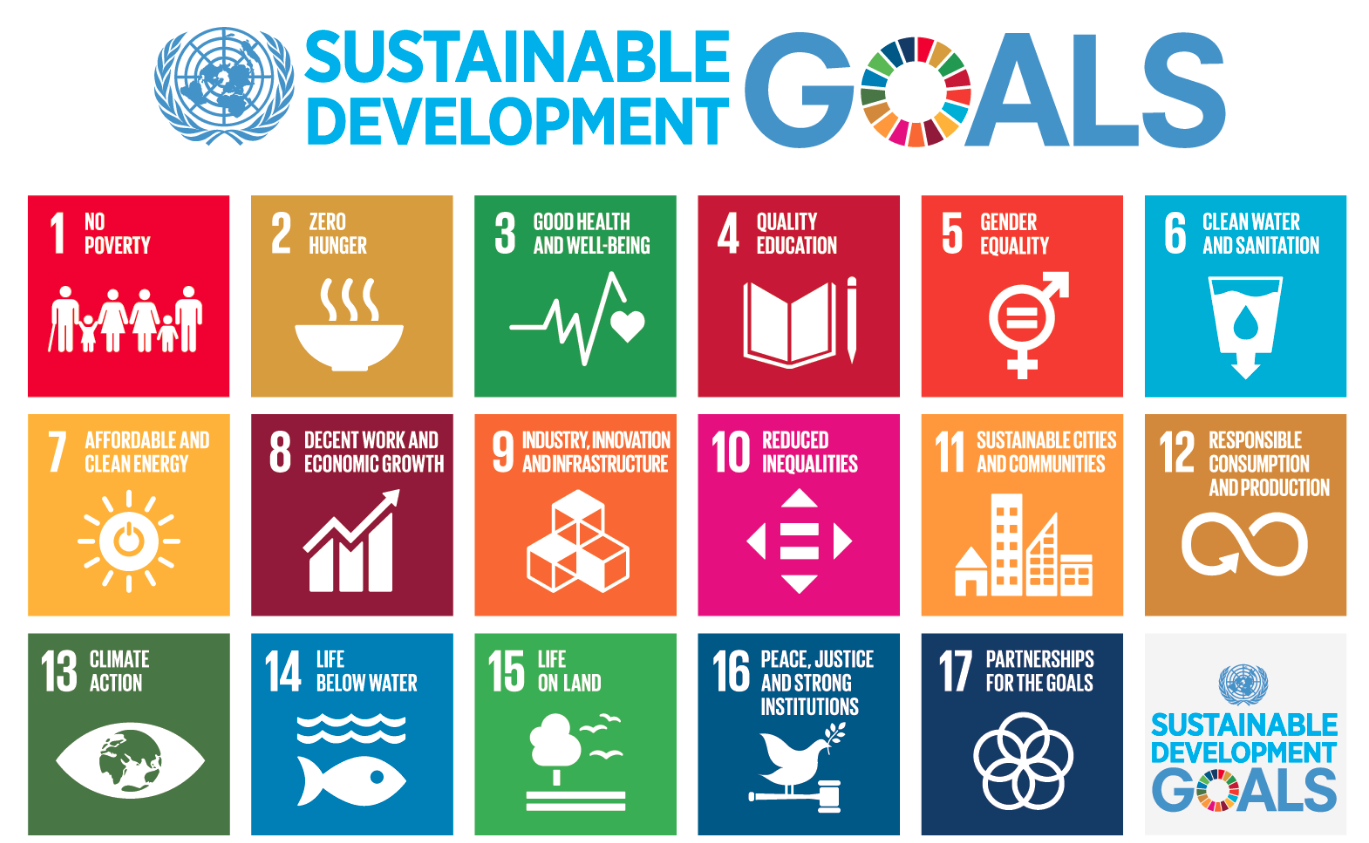
\includegraphics[scale=0.25]{Figures/chap2/SDG.png}
	\caption[United Nations Sustainable Development Goals]{United Nations Sustainable Development Goals}
	\label{fig:sdgs}
\end{figure}

The heightened importance of sustainability is evident both in the elevation of the word to the collective title of the \acp{sdg}, but also in the increased frequency of its use within the goals. In the original \acp{mdg} the word "sustainable" or a variant thereof is used only once in the goals and 6 times among the targets and indicators (and even then it is most commonly in reference to "debt sustainability"). In the \acp{sdg}, "sustainable" and its variants is found 13 times in the goals and 68 times among the targets and indicators, referring to a whole host of domains but most commonly referring to "sustainable development" or sustainable use of various resources. While significant gaps in our understanding and recognition of the connections between the environment, human wellbeing, technologies, and decision-making persist \cite{bennichDecipheringScientificLiterature2020}, the \acp{sdg} are a notable step towards acknowledging that our planet is one complex system and that, in many cases, attempts to tackle one domain without considering the others are fated to fail. 

Despite their short, clear formulations, actually achieving many of the \acp{sdg} involves the significant work by numerous actors in many domains and involving various technologies, as evidenced by the total of 169 targets and  232 indicators within the goals \cite{unitednationsgeneralassemblyGlobalIndicatorFramework2017}. In short, they require either the creation or the improvement of complex \ac{sts}. Within \ac{sdg} \#2, for instance, is Target 2.3: "By 2030, double the agricultural productivity and incomes of small-scale food producers, in particular women, indigenous peoples, family farmers, pastoralists and fishers, including through secure and equal access to land, other productive resources and inputs, knowledge, financial services, markets and opportunities for value addition and non-farm employment." Associated with this target are indicators 2.3.1, "Volume of production per labour unit by classes of farming/pastoral/forestry enterprise size," and 2.3.2, "Average income of small-scale food producers, by sex and indigenous status" \cite{unitednationsgeneralassemblyGlobalIndicatorFramework2017}. Clearly, accomplishing this goal will require innovation in agricultural technology, creation of new policy and technological mechanisms for linking financial services to these small-scale food producers, and new methods of collecting information to enable both the evaluation of our progress and the \ac{sts} created to reach the target. 

It is at this need that the research questions of this thesis are addressed.

\subsection{\hlc[green]{Why Systems Engineering?}} \label{sec:se}

Before answering this section's title question, we must first offer an a definition of systems engineering, as, unlike many other fields of engineering (aerospace, mechanical, electrical, biomedical, etc.) the name is not self-explanatory. 

Systems engineering, perhaps due to its inherently interdisciplinary nature coupled with its roots in several different fields (aerospace engineering, civil engineering, mechanical engineering, etc.), has had numerous definitions proposed over the course of the past century. Some of these have been by individual authors, such as Maier and Rechtin's "\textit{A multidisciplinary engineering discipline in which decisions and designs are based on their effect on the system as a whole}" \cite{maierArtSystemsArchitecting2009}, and some by international standards organizations, such as the \ac{iso}/\ac{iec}/\ac{ieee} definition "\textit{Interdisciplinary approach governing the total technical and managerial effort required to transform a set of customer needs, expectations, and constraints into a solution and to support that solution throughout its life}" \cite{internationalorganizationforstandardizationSystemsSoftwareEngineering2010} . For the purposes of this discussion, the specific definition is not overly important, as we do not seek to create a foundational work of systems engineering, but rather to understand its relations to other fields.

It is worth noting \ac{incose} affiliated \ac{sebok} definition, however: "Systems Engineering is an interdisciplinary approach and means to enable the realization of successful systems. It focuses on holistically and concurrently understanding stakeholder needs; exploring opportunities; documenting requirements; and synthesizing, verifying, validating, and evolving solutions while considering the complete problem, from system concept exploration through system disposal" \cite{systemsengineeringbodyofknowledgeSystemsEngineeringGlossary2021}. Something missing from this definition is that systems engineering refers to a specific intellectual tradition that arose out of mechanical, civil, electrical, and aerospace engineering fields in the early-to-mid 20th century. It thus tends to draw from an engineering mindset and relies upon engineering techniques, rather than those of urban planning, architecture, or program management, all of which also could be considered to fall into the \ac{sebok} definition. This is important because the nature of systems engineering is that it is inherently abstracted from its subject matter to a certain degree. The tools of systems engineering were developed in order to design hydroelectric dams, rockets, global communications systems, and much more. In this way it is similar to control theory, in that is is not deeply tied to the specific thing being designed or controlled, only to an abstract understanding of its mechanics and relationships. This means that systems engineers, like some physicists, can have a tendency to see any problem, any situation as tractable with a systems engineering perspective.

So with some shared understanding of what systems engineering is established, why is it relevant to sustainable development? First and foremost, it is the `interdisciplinary' and `holistic' nature of the field, along with the tools and frameworks that have been developed to apply this, that makes it most relevant for \ac{evdt}. While sustainable development and engineering historically have not been viewed as closely linked, this is changing. Sustainability first enters engineering literature in the 1970s and its frequency rises in a logarithmic fashion over the course of the subsequent decades \cite{deweckInvestigatingRelationshipsSemantic2012}.

The primary systems engineering tools of interest include the aforementioned multidisciplinary optimization, which provides lessons on integrating models of different fields; systems architecture, which is useful for designing \ac{evdt} implementations themselves; and stakeholder analysis, as all \ac{evdt} applications inherently involve numerous stakeholders, often with different levels of power. 

Other subfields that will be relevant later in the \ac{evdt} lifecycle include multi-stakeholder negotiation and decision-making, which contains numerous lessons on how structure communications to avoid deadlock or domination \cite{fitzgeraldEffectsEnhancedMultiparty2015,fitzgeraldRecommendationsFramingMultistakeholder2016,weckMULTISTAKEHOLDERSIMULATIONGAMING2012}; tradespace visualization and exploration \cite{fitzgeraldEffectsEnhancedMultiparty2015,fitzgeraldRecommendationsFramingMultistakeholder2016,groganInteractiveModelsSystem2015,rossMultiAttributeTradespaceExploration2004,selvavaleroRulebasedSystemArchitecting2012}, which contains lessons on how to present complex information to stakeholders and enable them to navigate their options; and epoch-era analysis, which is useful to considering how a system may evolve over time in an high uncertainty domain \cite{rossUsingNaturalValueCentric2008,vascikMethodExploringProgram2015}. Sachs stated that "Sustainable development is also a science of complex systems" and argued that two specific tools are important for implementing the \acp{sdg}: backcasting and technology road-mapping \cite{sachsAgeSustainableDevelopment2015}. Systems engineering is well equipped to address both of these.


External to the field itself, the rise of sustainable development, with its interconnected social, economic, and environmental development, has also been paralleled by the (rightfully) expanded number of stakeholders involved in decision-making processes and a increased recognition of linkages across differing geographic scales \cite{brommelstroetPlanningSupportSystems2010}. This increase in complexity is something that systems engineering is well posed to address.

%The growth and development of cities is a complex system. Much work has been done using cellular automata and fractals to model them \cite{battyCitiesComplexity2005}

%Urban planners have been seeking to develop useful indices and indicators akin to those used in engineering and remote observation contexts for decades (Section 1, Cahpter 3 of \cite{boyceFrameworkDefiningApplying1972}


%"Futures planning as described and prescribed by futurists is different from planning \textit{for} te future; it is an attempt to manipulate or plan \textit{the} future. A basic characteristic of this orientation is the use of such terms as "designing," "inventing," or even "making" the future. When the future is being planned for, rather than designed, the implication is that the planner is trying to make specific and limited accomodations to the broad and overall characteristics of the future he considers either immutable or too formidable to be fundamentally rearranged or restructured" \cite{robinsonDecisionmakingUrbanPlanning1972}.
%
%"If alternatives are not carefully related to goals and objectives there is the real danger that they will either fail to reflect certain important issues which the planning process to being used to study, or worse still, be almost irrelevant... Alternatives must reflect the goals sought; the means must reflect the ends" \cite{mcloughlinChartingPossibleCourses1972}.
%
%
%
%This work does not directly incorporate mechanisms for multi-stakeholder negotiation or tradespace exploration, but it is amenable to extension with such mechanisms (refer to SEAri research). The importance of multicriterion choice has been evident in planning applications since the early days of \ac{gis}, and Jankowski porposed a framework for accomplishing this \cite{jankowskiIntegratingGeographicalInformation1995}. Many of the early attempts in this direction focused on the use of linear weighted combinations of the criteria to form a single utility function \cite{malczewskiGISbasedApproachMultiple1996}.	

%Refer to epoch-era analysis and tie that in to scenario planning history.

\subsection{\hlc[green]{Why Remote Observation and Earth Observation Data?}} \label{sec:remote}

Remote observation, often used interchangeably with remote sensing, refers to any form of data collection that takes place at some remote distance from the subject matter \cite{jensenRemoteSensingEnvironment2006}. The term is fundamentally about \textit{how} the observation is taking place rather than \textit{what} is being observed, as it includes both astronomical telescopes and aircraft-based surveys of farmland. While there is no specific distance determining whether a collector is `remote,' in practice this tends to mean some distance of more than a quarter of a kilometer. Handheld infrared measurement devices are thus usually excluded (and thereby classified as \textit{in-situ} observations. Aerial and satellite imagery are definitively in the remote observation category. Low altitude drone imagery, particularly when the operator is standing in the field of view, is a gray area that is not well categorized at this time.

\Acf{eo} meanwhile is, as defined by \ac{geo}, the data and information collected about our planet, whether atmospheric, oceanic or terrestrial. This includes space-based or remotely-sensed data, as well as ground-based or in situ data \cite{grouponearthobservationsGEOGlance2019}. As defined by Mather and Koch, the interpretation and understanding of measurements of the Earth's land, ocean, or ice surfaces or within the atmosphere, together with the establishment of relationships between the measurements and the nature and distribution of phenomena on the Earth's surface or within the atmosphere \cite{matherComputerProcessingRemotelySensed2011}. \ac{eo} is thus the converse of remote observation, being determined by \textit{what} is being observed (the Earth), rather than \textit{how}. 

This thesis is primarily interested in the remote observation of the earth, and secondarily in other forms of \ac{eo} data. To that end, unless specified otherwise, the reader can assume that ``remote observation" and ``earth observation" both refer to ``remote observation of the earth."

While many of the initial efforts at remote observation from air and space were done with military objectives in mind, scientific, commercial, and social applications soon became abundant. Since much of space-based remote observation in the past several decades has been primarily driven by large governmental scientific organizations, much of that data has been made publicly available. An enormous amount of \ac{eo} satellite data is freely available to the public through 20+ \ac{nasa} earth science satellites \cite{shirahNASAEarthObserving2017}, the \ac{esa} Copernicus Programme (which includes both the 6 Sentinel satellites and in-situ measurements), the various satellites managed by the \ac{jaxa} \ac{eoc}, the \ac{cbers}, and the satellites of other space agencies. While this data is largely free currently, this has not consistently been true, nor is it guaranteed to continue in the future \cite{borowitzOpenSpaceGlobal2017}. For most of the early history of satellite observation, imagery was kept highly classified and zealously guarded, to the extent that Congressman George Brown Jr., who was integral in the establishment of the US \ac{ostp}, the \ac{epa}, and the \ac{ota}, resigned from his post on the House Intelligence Panel in protest over the enforced secrecy in even discussing the topic \cite{healyRepBrownQuits1987, barry1992mappings}. Even when the data was available to the public, it was not always freely available, as various countries have made attempts to monetize remote observation data. In the 1970s and early 1980s, for instance, Landsat data was a government-managed operation that provided products at a low-cost, based primarily on the cost of reproduction. In the 1980s, however, the program was transferred to a private entity and prices were increased by more than an order of magnitude and significant copyright restrictions were put in place \cite{mchaffieManufacturingMetaphors1994}. Currently the data is once again made free after the monetization efforts met with limited success \cite{waldropLandsatCommercializationStumbles1987}, but this may not remain the case moving forward \cite{popkinUSGovernmentConsiders2018}.

The use patterns of remote observation data has varied for reasons beyond cost and military secrecy, however. Social applications were being considered from quite early on. As Jennifer Light recorded, "one proponent [from the last 1940s] explained, photointerpretation data did not directly provide `social data,' yet they were `pertinent to social research needs in so far as such `physical data' have meaningful sociological correlates" \cite{lightWarfareWelfareDefense2005}. In the succeeding decades, the degree to which humans have altered the surface of our planet has only increased and, as a result, we can now also infer a great deal more about humans from images of that surface. By the early 1970s five rationales for using satellite imagery in city planing had become widespread \cite{lightWarfareWelfareDefense2005}:

\begin{enumerate}[itemsep=0pt,parsep=0pt]
	\item{It offers a synoptic, total view of the complex system in a given area.}
	\item{Satellites provide repetitive, longitudinal coverage.}
	\item{Satellite inventories were more efficient and up-to-date than ground surveys.}
	\item{Remote sensing was objective.}
	\item{Satellites produced digital imagery that could be easily combined with ground-based data in novel \acp{gis}.}
\end{enumerate}

Despite these rationales, cities and metropolitan areas largely elected not to use satellite imagery for several decades, choosing instead to rely on aerial imagery and ground-based surveys \cite{lightWarfareWelfareDefense2005}. The reasons for this are many, but probably include that many of these rationales were overstated for their day. Insufficient resolution and inconsistent coverage limited intra-urban use. While satellite imagery provides a wonderful decades-long longitudinal dataset now, it did not at the time. Satellite imagery was still heavily dependent on human photointerpretation, undermining the argument that the data was "objective" in any meaningful sense. Finally the cost and specialization required to effectively use the data limited its ability to be combined with other datasets. Black-and-white aerial imagery provided sufficient resolution, oblique angles, and immediate interpretability to even the untrained eye. Plus cities were compact enough that the advantages of scale offered by satellites largely did not come into play. Ultimately, while GIS technology (discussed in Section \ref{sec:gis}) was readily adopted by cities, satellite imagery was not \cite{lightWarfareWelfareDefense2005}.

Furthermore, despite espousing these five rationales, \ac{nasa} "did not go a long way toward incorporating remote sensing into day-to-day practices in city planning agencies. This was compounded by the fact that far more academics than local government officials participated in these experiments, providing applications of satellite data that were almost always a step removed from urban mangers' needs" \cite{lightWarfareWelfareDefense2005}. One of the first use of non-visual imagery for such applications, for example, was unaffiliated with \ac{nasa} or the space industry in general. In 1970, the city of Los Angeles used aerial infrared imagery to identify unsound housing, and, by 1972, had integrated this imagery with other datasets into a digital decision support system for assessing urban blight \cite{lightWarfareWelfareDefense2005}.

However, much as changed since the 1970s. The rise of multiple \ac{eo} satellite companies, including the company Planet's 100+ satellites \cite{tepperSatelliteMakerPlanet2015}, Digital Global's WorldView satellites, and Astro Digital’s recent launch of their first two satellites \cite{shieberAstroDigitalLaunched2017}, suggests that yet more satellite data is soon to be available for a price. These data sources are likely to be complimentary, with the commercial satellites primarily providing visual imagery and \ac{nasa} satellites primarily supplying other forms of scientific data, though the \ac{modis}, the \ac{viirs}, and the Landsat program all capture visual imagery as well. The launch of Sentinel-1 and other \ac{sar} satellites has enabled the monitoring of flooding through hurricane cloud cover \cite{zhangMappingExtentMagnitude2018}. While many of these satellites were designed primarily with scientific purposes in mind, this data is increasingly being used by a wide variety of groups around the world to enable sustainable development and other humanitarian applications, such as forest fire tracking [via \ac{modis} and \ac{viirs} \cite{schroederNewVIIRS375m2014}], agricultural monitoring [via \ac{gpm} for rainfall \cite{houGlobalPrecipitationMeasurement2014} and GRACE for soil moisture \cite{wahrTimevariableGravityGRACE2004}], climate change vulnerability assessments [via \ac{icesat2} for vegetation and ice monitoring \cite{mcgillMultipleAltimeterBeam2013}], and monitoring military actions [via Sentinel-1 \cite{sanchezSARSupportWar2022}].

Furthermore, over the course of the past two decades, efforts have been made to systematize the application of remote sensing data to inform decision-making on a host of sustainable development areas. Internationally, over 100 countries worked together to form the \ac{geo}\footnote{\ac{geo}, as the name suggests, is dedicated to Earth observation and specifically to the development of a \ac{geoss}. In practice this means working together to identify gaps in earth observation and reduce duplication, particularly surrounding sustainable development. In addition to the 100+ national governments, it also includes more than 100 so-called "participating organizations" which include space agencies, \acp{ngo}, professional societies, and multiple arms of the \ac{un}. For more information see \url{https://earthobservations.org/}.} and 60 agencies with active earth observation satellites have formed the \ac{ceos}\footnote{\ac{ceos} predates \ac{geo} and was pivotal in its creation. Regular membership is primarily restricted to space agencies that operate \ac{eo} satellites (though other organizations can join as associate members) and its activities tend to focus on interoperability and harmonization. Unlike \ac{geo}, all associate members are either government agencies or arms of the \ac{un}. For more information, see \url{https://ceos.org/}.}. In the US, the primary source of government funding for such applications is the \ac{nasa} Applied Sciences Program, a part of the Earth Science Division, that includes programs focused on disasters, ecological forecasting, health \& air quality, water resources, and wildland fires, using data from \ac{nasa} satellites as well as those of the \ac{usgs} and the \ac{noaa} \cite{khanLongHardJourney2009, nasaappliedsciencesprogramWhatWeNASA, nasaearthscienceappliedsciencesNASAAppliedSciences2021}. The Applied Sciences Program has clearly learned from \ac{nasa} past failures of engagement with local decision-makers, and now publish guides on how to ensure that new projects are actually helpful to users \cite{irwinSERVIRServicePlanning2017}. In keeping with this new mentality, the Applied Sciences Program, through their Capacity Building portfolio, frequently partners with other organizations, such as \ac{usaid}. For instance, both groups worked together to form the \ac{servir}, which provides geospatial information and predictive models to parts of Africa, Asia, Latin America. In a similar collaborative effort, \ac{nasa} and \ac{usaid} have also integrated remote sensing data into the \ac{fews}. 

Such efforts have been quite successful in their goals, but have required significant time, expertise, and effort to create and maintain. As overpass frequencies, resolutions, and computational speed have increased, it is increasingly possible to conduct much more rapid, localized, and ad hoc applications of remote sensing data for sustainable development and humanitarian purposes. Within 48 hours and one week respectively, \ac{nasa} was able to provide maps of damaged areas of Mexico City to Mexican authorities following the 2017 earthquake \cite{nasajetpropulsionlaboratorySatelliteRadarDetects2017} and maps of damaged areas of Puerto Rico to the \ac{fema} following Hurricane Maria \cite{nasajetpropulsionlaboratorySatelliteDataPuerto2017} (in fact, both of these maps were provided during the same week), through \ac{nasa}'s Disasters Team under the Applied Sciences Program. Such data collection and processing can increasingly be done without the expertise and remote observation systems of governmental space agencies, as demonstrated by a recent effort to conduct near-real-time deforestation monitoring and response \cite{finerCombatingDeforestationSatellite2018}.

These developments have powerful implications for equity. "The geography agenda is distorted by being data-led... The first law of geographical information: the poorer the country, the less and the worse the data"  (\cite{overton1991further} as paraphrased by \cite{taylorGeographicInformationSystems1994}). Remote observation has the potential to help upend this, by providing at least some base level of data globally, with no distinctions of borders or wealth. Increasingly, sustainable development applications of remote observation data are not limited by available remote observation platforms, but by lack of knowledge by potential end-users of its value and by the tools to make use of available data. While data is often available (either freely or at some cost), it is not always readily accessible (particularly in real time) or easily interpreted. Those with the knowledge and capabilities to access and transform this data continue to reside primarily in government agencies and universities (though we have certainly seen heartening growth of such users in a much more diverse set of countries over the past couple of decades). The majority of prominent \acp{eos} are still designed primarily with scientific, meteorological, or military purposes in mind, limiting their utility in more applied contexts, regardless of the creativity of users. And many successful applications of \ac{eo} data, particularly that which is not straightforward visual imagery, remain squarely focused on characterizing specific, usually environmental, phenomena, such as wildfires \cite{schroederNewVIIRS375m2014},  aquatic bacterial growths \cite{stromingQuantifyingHumanHealth2020}, or deforestation \cite{lagomasinoMeasuringMangroveCarbon2019}, with only limited excursions into assessing the connections between such phenomena and human wellbeing. For a survey of such applications see \cite{southernhemispheresummerspaceprogram2013CommonHorizonsWhite2013}.

One important exception to generalization is the recent development of critical remote sensing. This field, most clearly laid out by Bennet et al. reconsiders the rationales for the use of satellite data discussed above in a more critical light \cite{bennettPoliticsPixelsReview2022}. In particular, they advocate for a tripartite research agenda of \textit{exposing}, \textit{engaging}, and \textit{empowering}. By exposing, they mean using remote sensing to provide evidence of socioeconomic and environmental injustices, with a particular emphasis on clandestine activities. By engaging, they mean recognizing the very much non-objective perspective of remote sensing and seeking to integrate remote sensing with local knowledge rather than supplant it. By empowering, they mean partnering with groups that remote sensing is collecting data about, particularly marginalized groups, for capacity building and participating in the use of the data.

As stated in the \textit{Common Horizons} report, "space technology provides awareness of how the sustainability of the world is affected and contributes to its improvement" \cite{southernhemispheresummerspaceprogram2013CommonHorizonsWhite2013}. Due to the potential of such technologies for applications in humanitarian and sustainable development, attempts are starting to be made to quantify the value of various earth observation systems, but many of these have been limited by the inherent difficulties of handling counterfactual scenarios \cite{macauleyValueInformationMeasuring2006}. \ac{nasa} is well aware of this difficulty, which is why the Applied Sciences Program funded the \ac{valuables} at \ac{rff}. This consortium is using economic methods to improve estimates of the societal benefits of earth observation. Work by \ac{valuables} and others has quantified the value of remote observation systems for carbon emission tracking \cite{cookeUsingSocialCost2016}, agricultural production \cite{forneyEconomicValueRemoteSensing2012}, and ground water quality \cite{forneyEconomicValueRemoteSensing2012}. Siddiqi et al. meanwhile have sought to incorporate data uncertainty and quality into estimates of satellites value for decision-making \cite{siddiqiIntegratingGloballyDispersed2020, siddiqiValuingRadiometricQuality2021}. The recent advances in this field are cataloged in the recent publication of a book on the socioeconomic value of geospatial information (which includes more than remote observation) \cite{kruseGEOValueSocioeconomicValue2017}. Integrating econometric models with remote observation system models is useful for both assessing the impact of past missions and for predicting the impact of future ones. Such results can be used to help justify the field as a whole and specific remote observation systems in particular. Many applications, however, require more detailed models that integrate more domains. This is particularly true if the intent is to provide remote observation data to inform operational decision-making.

More is needed to enable the use of \ac{eo} data for human decision-making in such a way that acknowledges the linkages between the environment and humans. This is major aim of this work. 

\subsection{\hlc[green]{Why GIS?}} \label{sec:gis}

The term \ac{gis} refers to any digital system for storing, visualizing, and analyzing geospatial data, that is data that has some geographic component. It can be used to discuss specific systems, a method that uses such systems, a field of studying focusing on or involving such systems, or even the set of institutions and social practices that make use of such a system \cite{sheppardGISSocietyResearch1995}. This may seem vague, but due to the diversity of its use, it is difficulty to hammer out a more specific definition without excluding important aspects \cite{goodchildOverviewDefinitionGIS1992, picklesToolScienceGIS1997, chrismanWhatDoesGIS1999, heikkilaGISDeadLong1998}. One perspective, however, is to view \ac{gis} to the underlying computer systems enabling the middle three components of the broader \ac{gisc} methodology, as shown in Figure \ref{fig:boundaries}. In that sense, the work related in this thesis can be seen as an exercise in \ac{gisc} spanning all five components, while the specific software produced for this work are instances of \ac{gis}. It should be noted that this distinction is not commonly made outside of academia, with \ac{gis} commonly being used generically to encompass both \ac{gisc} and \ac{gis}. Along these lines, there being some debate about whether \ac{gis} is best viewed as a scientific field in its own right, or as a mere tool for use in various other fields of science (such as environmental science, economics, etc.) \cite{goodchildGeographicalInformationScience1992,goodchildTwentyYearsProgress2010}. One important aspect of the 
ac{gisc} perspective that is not included in Figure \ref{fig:boundaries}, is that includes "institutional, managerial, and ethical issues \cite{goodchildGeographicalInformationScience1992}, something that is naturally core to this work. 

Data maps have a long history. Tufte dates them to the seventeenth century and cites Edmond Halley's 1686 chart of trade winds as "one of the first data maps" \cite{tufteVisualDisplayQuantitative2001} though arguably Scheiner's 1626 sunspot visualization qualifies as a data map \cite{friendlyBriefHistoryData2008}, as perhaps do Polynesian knot maps, which long predates either \cite{davenportMarshallIslandsNavigational1960}. Graphing data over time, meanwhile dates by to the 14th century \cite{friendlyBriefHistoryData2008}.

The term \ac{gis} and the associated field of study originated in the 1960s and 70s with experimental efforts of the Canada Geographic Information System and the US Bureau of the Census to digitize their demographic and land cover data \cite{goodchildGeographicInformationSystems1994}. It should be noted that these early instances were primarily application, rather than technology driven \cite{goodchildGeographicalInformationScience1992}. The key value of \ac{gis} is that it "allows geographers to integrate diverse types of data over different spatial scales from the regional to the global, while the advanced capabilities of GIS for organizing and displaying these data transform the geographer's view of the world" (\cite{tomlinsonPRESIDENTIALADDRESSGEOGRAPHIC1989} as paraphrased in \cite{vereginComputerInnovationAdoption1994}).

\begin{figure}[h]
	\centering
	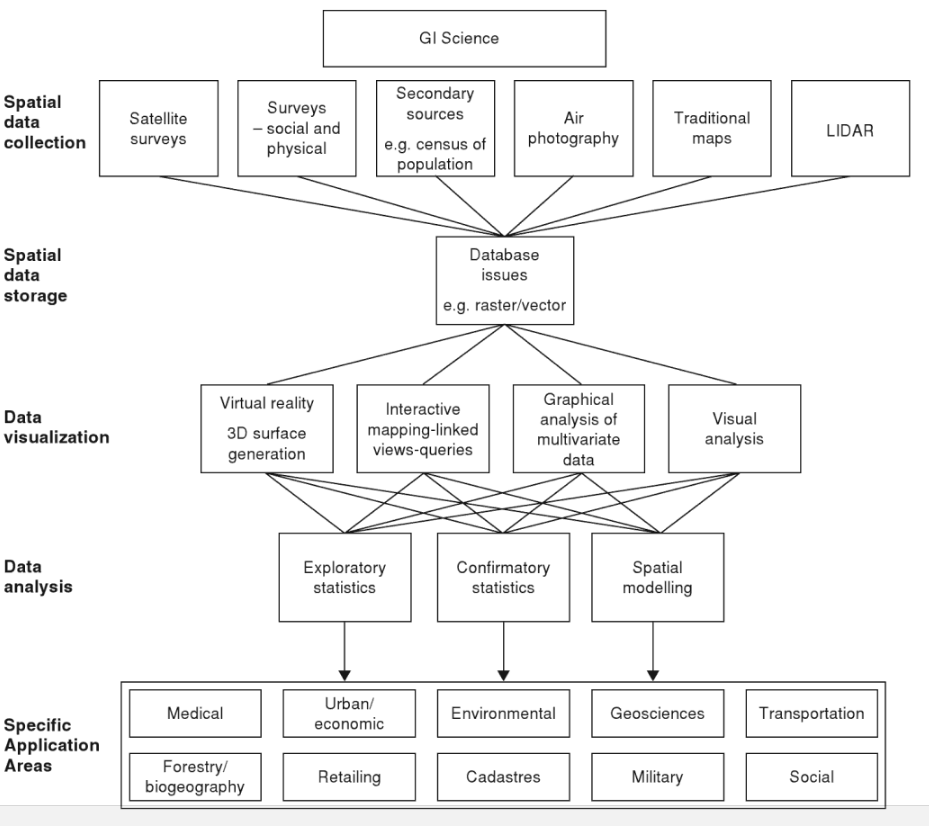
\includegraphics[scale=0.4]{Figures/chap2/GIScience.png}
	\caption[Overview of Geographical Information Science]{Overview of Geographical Information Science. From \cite{fotheringhamGeographicInformationScience2007}}
	\label{fig:giscience}
\end{figure}

Even with the relatively limited computing capabilities of the era, interest in \ac{gis} grew quickly with local governments quickly adopting it for planning purposes, as was mentioned in Section \ref{sec:remote}. One key moment in the development of \ac{gis} as we know it, was ESRI's creation of the shapefile format (which links geometries with data in a standardized, if somewhat limited, fashion) in the late 1980s, and, more importantly, their open publishing of the format, allowing others to create and manipulate such files \cite{goodchildModelingEarth2011}. In 1990, Tomlin defined the sub-discipline of \ac{gis} known as cartographic modeling, which attempts to generalize and standardize the analytic and synthetic capabilities of geographical information systems. It does so by decomposing data, data-processing tasks, and data-processing control notation into elementary components that can be recomposed with relative ease and great flexibility" \cite{tomlinGISCartographicModeling2012}. This theory would come to underlay much of research and development work done with \ac{gis}. including that of this thesis. 

With the development of \ac{gis} and the proliferation of its uses came the realization that no one single type of data field model could serve all needs. In 1991, Goodchild defined six different \ac{gis} data field model types and states that "no current \ac{gis} gives its users full access to all six" \cite{maguireGeographicalInformationSystems1991}:

\begin{enumerate}
    \setlength{\itemsep}{0pt}%
    \setlength{\parskip}{0pt}%
	\item{Sample randomly located points (e.g. weather stations, \ac{lidar} data)}
	\item{Sample randomly from a grid of regularly space points (e.g. many data validation studies}
	\item{Divide the area into a grid in which each rectangular cell records the average, total, or dominant value; i.e. raster data (e.g. satellite imagery)}
	\item{Divide the area into homogenous regions and record the average, total, or dominant value in each area (e.g. census data, soil maps)}
	\item{Record the locations of lines of fixed values (e.g. contour or isopleth maps}
	\item{Divide the area into irregular shaped triangles and assume the field varies linearly within each (e.g. some \acp{dem})}
\end{enumerate}

The aforementioned ESRI shapefiles are commonly used to store data of types 1 and 4, but is limited in its ability to store the others in an efficient manner. Such limitations are by no means unique to shapefiles. During the mid 90s, Goodchild noted that the field of \ac{gis} in general had several shortcomings \cite{goodchildGeographicInformationSystems1994}:

\begin{itemize}
    \setlength{\itemsep}{0pt}%
    \setlength{\parskip}{0pt}%
	\item{Two-dimensional, with some excursions into three}
	\item{Static, with some limited support for time dependence}
	\item{Limited capabilities for representing forms of interaction between objects}
	\item{A diverse and confusing set of data models}
	\item{Dominated by the map metaphor}
\end{itemize}

To some extent, many of these issues, such as the lack of three dimensional systems, persisted well past the 90s \cite{goodchildTwentyYearsProgress2010}. Despite this, by 1991, Maguire et al. felt that "it is not fanciful to suggest that by the end of the century GIS will be used every day by everyone in the developed world for routine operations" \cite{maguireGeographicalInformationSystems1991}. This, of course, would turn out to be an understatement, as the world is currently incredibly dependent on \ac{gis}. Individuals rely upon the various map applications that we use to search and navigate our world. Governments use maps to visualize their jurisdictions and motivate action, as Chicago has done by visualizing food deserts and mapping where new supermarkets are both needed and economically viable \cite{goldsmithResponsiveCityEngaging2014}. Since the turn of the millennium, spatial data has become deeply ingrained economics, urban studies, private industry, social networks, environmental science, public health, criminal justice, and more \cite{goodchildSpatiallyIntegratedSocial2000}.

There is now a well established marketplace for geographic data (as shown in \ref{fig:marketplace}) and thus for \acp{gis} to handle that data. It should be noted that the institution that I am associated with, a university, is classified here as a "value-added intermediary" which serves an important connective role between suppliers, infrastructure, and users. This positioning is crucial to the nature of this work. Whether one is interested in remote observation data or local economics, the question is not whether one should use \ac{gis}, but how. To this end, the next two sections will go into more detail about two different veins of \ac{gis}: collaborative systems and decision support systems.

\begin{figure}[h]
	\centering
	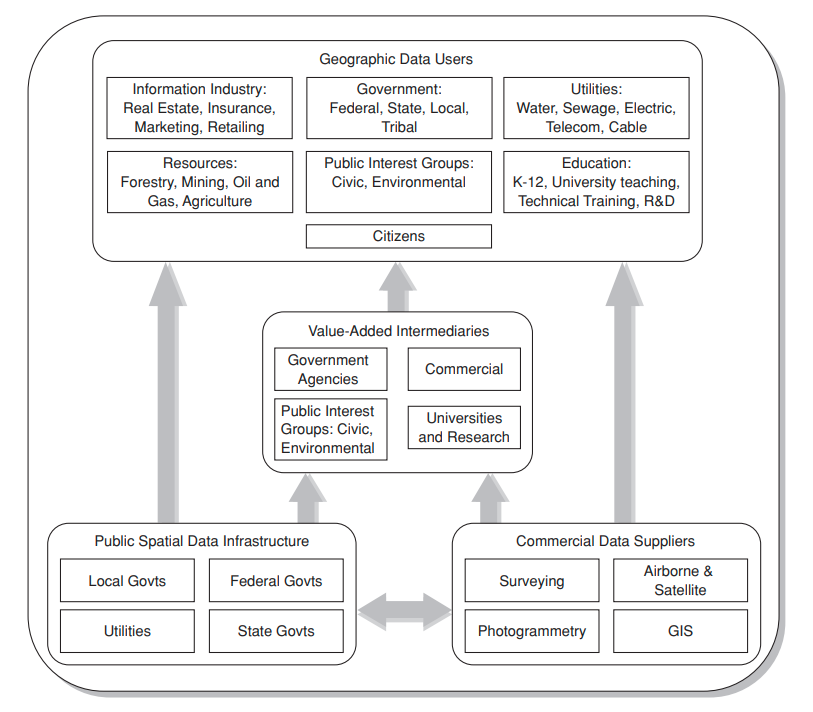
\includegraphics[scale=0.4]{Figures/chap2/GISMarketplace.png}
	\caption[The marketplace for geographic data]{The marketplace for geographic data. From \cite{cowenAvailabilityGeographicData2007}}
	\label{fig:marketplace}
\end{figure}

\subsection{\hlc[green]{Why Collaborative \& Open Source?}} \label{sec:collaborative}

As was mentioned in Section \ref{sec:remote}, many of the early applications of remote observation data were technology-driven rather than need-driven. So it was with the closely related field of \ac{gis} as well, leading to powerful critiques by Pickles and others \cite{picklesGroundTruthSocial1994}. These critiques resulted in a reconsideration of the top-down nature of the field and the identification of several potent reasons for broadening the base of participation. First, there was the recognition that the developer of a \ac{gis} is not the supreme authority on all fields. "It is the geomorphologist who is best able to choose the data model for representation of terrain in a GIS, not the computer scientist or the statistician, and it is the urban geographer who is best able to advice on how to represent the many facets of the urban environment in a GIS designed for urban planning" \cite{goodchildGeographicInformationSystems1994}. This means that, while collaborations certainly can introduce additional difficulties, such as cultural conflicts, issues of interpersonal trust, effort required to establish rules and norms of participation, they are also immensely rewarding and can improve the results of the work \cite{tullochInstitutionalGeographicInformation2007}. The dynamics at play in such collaborations can be seen in Figure \ref{fig:east2}. This is certainly a more complicated situation than the traditional, straightforward, academic implementation of a \ac{gis} project.

\begin{figure}[h]
	\centering
	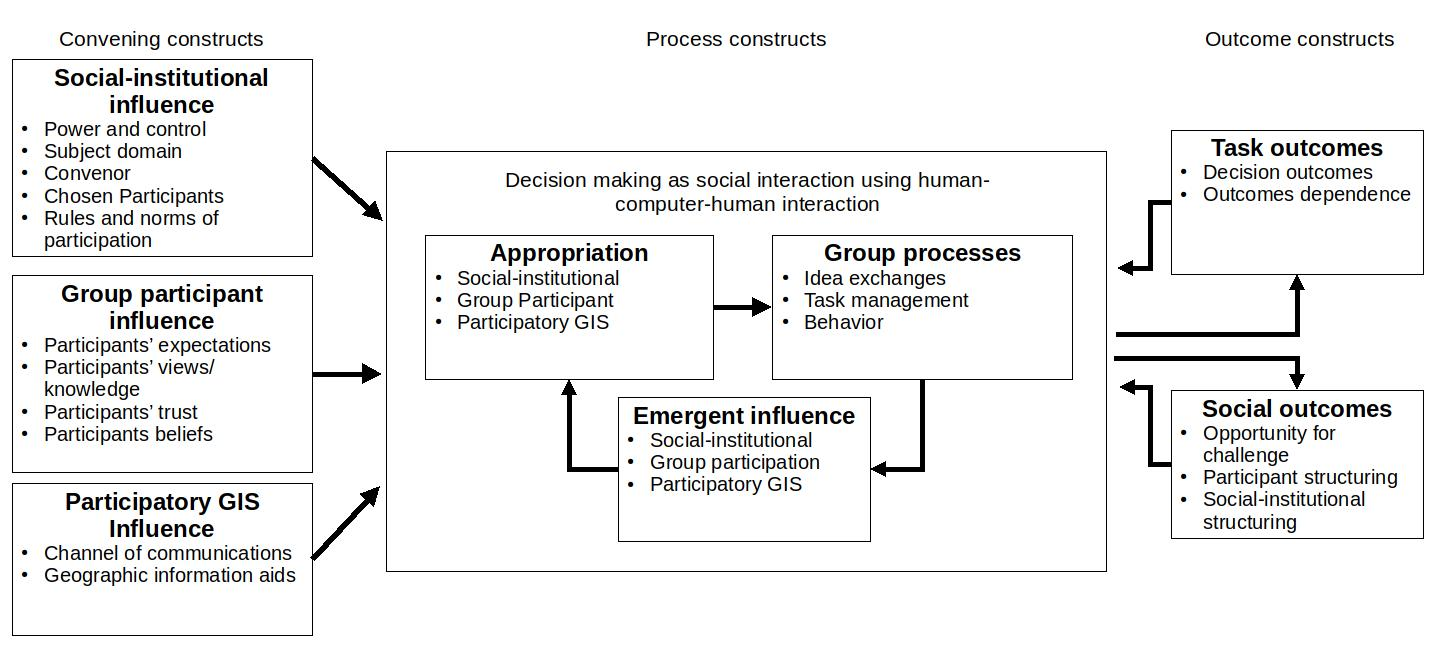
\includegraphics[scale=0.4]{Figures/chap2/east2.jpg}
	\caption[Enhanced Adaptive Structuration Theory 2]{Enhanced Adaptive Structuration Theory 2 (EAST2). Adapted from \cite{jankowskiGISGroupDecision2001}}
	\label{fig:east2}
\end{figure}

Second, there was a recognition of the equity concerns at play. Users and disadvantaged communities needed to be involved in the development of \ac{gis} data, analysis, and use, if they were going to have a meaningful chance of improving their circumstances \cite{talenBottomUpGIS2000}. The Canadian International Development Research Centre noted that, "It is impossible to have sustainable and equitable development without free access to reliable and accurate information" \cite{benmouffokInformationDecisionMaking1993}. Meanwhile, academic geographer Matthew Edney argued that, "Without equitable access to GIS data and technology, small users, local governments, nonprofit community agencies, and nonmainsream groups are significantly disadvantaged in their capacity to engage in the decision-making process" (\cite{edney1991strategies} as paraphrased in \cite{harrisPursuingSocialGoals1994}). Williams, in \textit{Data Action}, argues that since "data represents the ideologies of those who control it use," collaboration is essential for creating "trust and co-ownership in the data analysis by allowing the work to be critiqued by those who know the issue the best" and ensuring "that the voices of people represented in the data are neither marginalized nor left unheard."

There was thus reason to seek ways to overcoming the limitations of the technology which, as was common sentiment at the time, meant that "for billions the possibility of accessing the best technology and information made available through digital communications network will always be a luxury. Cartographic information, digital or otherwise, becomes a commodity in its mass production and marketing" \cite{mchaffieManufacturingMetaphors1994}. 

In the early 2000s, this desire motivated the growth in interest towards deconstructing current practices and expanding participation. Several names and frameworks were proposed, including Bottoms Up GIS \cite{talenBottomUpGIS2000}, critical cartography \cite{cramptonIntroductionCriticalCartography2005, kimCriticalCartographyParticipatory2015}, GIS and Society \cite{sieberPublicParticipationGeographic2006}, and \ac{ppgis}. The last of these, which sought to directly involve the public, would become the most widely used, and would be associated with the broader field of \ac{pgis} \cite{sieberPublicParticipationGeographic2006}, which also included other stakeholders, including government officials, \acp{ngo}, private corporations, etc. More recently these lesson from \ac{gis} have been incorporated with similar lessons from other data science and design fields to form methodologies and approaches such as Data Action \cite{williamsDataActionUsing2020}, Data Feminism \cite{dignazioDataFeminism2020}, and Design Justice \cite{costanza-chockDesignJusticeCommunityLed2020}. It should be noted that these fields seek involvement in both the production of data and in its application, not merely one or the other \cite{weinerParticipatoryGeographicInformation2007, talenBottomUpGIS2000}. For example, in Washington state in 2002, several American Indian tribes were using \ac{gis} technology to "inventory, analyze, map, and make decisions regarding tribal resources... include[ing] timber production, grazing and farm land, water rights, wildlife, native plants, cultural sites, environmental data and hazardous site monitoring, historical preservation, health and human resources" \cite{bondCherokeeNationTribal2002}. And in 1999, the 'What If?' \ac{pss} was created to use "GIS data sets that communities have already developed to support community-based efforts to evaluate the likely implications of alternative public-policy choices" \cite{klostermanWhatIfCollaborative1999}. 

This dual involvement promotes, as Michael Curry put it, both "knowing \textit{how}" (the "ability to do something") and "knowing \textit{that}" (the "knowledge about how something works") \cite{curryGeographicalInformationSystems1994}. Having only the former forces the user to rely upon blind trust, instilling a sense of complacency or alienation and preventing creativity. Knowing only the latter, enables discourse about a topic but prevents the user from actually implementing new ideas. It is only with both together that a person becomes a true participant in a field and make their own choices. This is important as expansion of choice is valuable for both intrinsic (for its own sake) and instrumental (to attain preferred positions) reasons \cite{senFreedomChoiceConcept1988}.

\ac{pgis} has thus naturally been strongly advocated and widely adopted over the past three decades \cite{drummondFutureGISPlanning2008}, with numerous frameworks being proposed for how to implement it \cite{brommelstroetPlanningSupportSystems2010}. A relatively early project in this vein, for example, sought to try and overcome issues of unequal access and use of \ac{gis} technology in South Africa in the early 1990s through the pursuit of five specific objectives \cite{harrisPursuingSocialGoals1994}: 

\begin{enumerate}[itemsep=0pt,parsep=0pt]
	\item{Enhanced community/development planner interaction in a research and policy agenda setting}
	\item{The integration of local knowledge with exogenous technical expertise.}
	\item{The spatial representation of relevant aspects of local knowledge.}
	\item{Genuine community access to, and use of, advanced technology for rural land reform.}
	\item{The education of "expert" rural land use planners about the importance of popular participation in policy formulation and implementation.}
\end{enumerate}

Such objectives are common across \ac{pgis} projects and the success of this pursuit has come to be recognized even by many entrenched institutionalists. The former vice-mayor of New York City, for instance, argues that digital \ac{gis} tools that provide open data (1) free data from bureaucratic constraints, allowing real time combination of data from different sources; (2) construct a loop between government and the community in which cooperation builds respect continuously; (3) enable two-way communication, promoting collaboration \cite{goldsmithResponsiveCityEngaging2014}. That said, some of these implementations have been criticized for being participative in name only, particularly within the research domain \cite{tebrommelstroetRelevanceResearchPlanning2009}.


Many \ac{pgis} implementations still rely upon closed source, proprietary code for the underlying software \cite{heikkilaGISDeadLong1998}. Participants made have been able to generate new data and perform analyses, but they often could not access the code itself or change the models directly. This was due to a combination of factors: limited diffusion of programming knowledge; a limited selection of software tools, many of which were closed source; limited access to computers and the internet; and limited collaboration tools, particularly for geographically distributed collaborations \cite{cramptonIntroductionCriticalCartography2005}. Over the past couple decades however, all three of these limitations have been greatly mitigated (though not eliminated), due to the growth of the internet and the related diffusion of programming knowledge and rise of the open source movement. As two leaders of the \textit{theirwork} \ac{ppgis} project in 2011 put it \cite{williamsonTheirworkDevelopmentSustainable2011}, 

\blockquote{The open source movement at its core stands for the development of source code... in a completely open and free way. Pragmatically, this manifests itself as a methodology of making code freely available to anyone who may wish to access it for any purpose, unconditionally. Concurrently, open source is for many a philosophical approach to software development, and is see as the only truly sustainable approach to software development... In both its execution as a model for making possible new forms of collaborative work, and its philosophical underpinnings of sustainability and openness, it is an essential component in and fluence upon a computer-based mapping solution.}

This passionate call for open source software is about more than a philosophical ethical stance. It is also about enabling critique and improvements. ``Map studies needs to open the `black boxes' of mapping software, to start to interrogate algorithms and databases, and in particular to investigate the production of ready-made maps that appear almost magically on the interfaces of gadgets and devices we carry and use everyday, often without much overt thought about how they work and whose map they project onto their interface" \cite{dodgeMappingModesMethods2011}.

It should be noted that some work has placed the responsibility for limited adoption of \ac{gis} tools on the planners/users themselves, specifically their lack of will and training with the tools \cite{gocmenBarriersGISUse2010}. While this may be the case, this lack of will and training is almost certainly itself due to a lack of outreach on behalf of the tool developers, and thus \ac{pgis} is still reasonable strategy to address these barriers. Other challenges around open source tools involve concerns about long-term support. As many (though certainly not all) open source projects are volunteer or academic-driven, changes of interest, financial support, or time availability can have major impacts on the software development and maintenance process. That said, similar concerns can be raised around commercial software products, which can be abruptly canceled, leaving the users with little recourse. It should be acknowledging that the economics, incentives, and decision-theory surrounding open source vs. closed source software is complex \cite{lernerSimpleEconomicsOpen2002}, but the continued endurance of open source software (or even thriving, as virtually all servers used for cloud computing are running on open source operating systems \cite{vermaUbuntuLinuxMost2015}), suggests that open source is a viable choice for software projects moving forward. 


\subsection{\hlc[cyan]{Why Decision Support \& Scenario Planning?}} \label{sec:scenario}

\subsubsection{\hlc[cyan]{Decision Support Systems}}

One common use of \ac{gis} is in \acp{dss}. These are technical systems aimed at facilitating and improving decision-making. Functions can include visualization of data, analysis of past data, simulations of future outcomes, and comparisons of options. Such \ac{gis} \acp{dss} are particularly common in development and planning spheres. Planning here refers to "the premeditation of action, in contrast to management [which is] the direct control of action" \cite{harrisLocationalModelsGeographic1993}. In general, planning tends to concern itself with more long-term affairs that management does. Planning strives for the "avoidance of unintended consequences while pursuing intended goals." Models, and their specific implementations as decision/planning support tools, are one means of achieving this. 

One of the chief reasons to use \acp{dss} is that singular optimal solutions to societal problems often either do not exist or are infeasible to calculate. For instance, even in the circumstance where economic welfare is agreed to be the primary or sole objective, in order for cost-benefit analysis to maximize economic welfare, the following conditions must be met \cite{krutillaWelfareAspectsBenefitCost1961}:

\begin{enumerate}[itemsep=0pt,parsep=0pt]
	\item{Opportunity costs are borne by beneficiaries in such way as to retain the initial income distribution.}
	\item{The initial income distribution is in some sense ``best."}
	\item{The marginal social rates of transformation between any two commodities are everywhere equal to their corresponding rates of substitution except for the area(s) justifying the intervention in question.}
\end{enumerate}

It is not often that all three conditions are met. More detailed modeling, as well as breaking down specific costs and benefits (as opposed to converting them to monetary terms and summing them) and attributing them to specific goals, can circumvent these constraints, though at the cost of increased complexity \cite{hillGoalsAchievementMatrixEvaluating1972}.

Meanwhile, the law of requisite variety from the field of cybernetics says that the variety (the number of elements or states) of the control device must be at least equal to that of the potential disturbances to the system \cite{ashbyRequisiteVarietyIts1991}. Any development plan is going to fall far short of the variety expressed by human society and the natural environment. Planning efforts must then make reliance on the natural homeostasis behavior of such systems and of more flexible, ad hoc measures not specified in the plan in order to make up the difference in variety \cite{mcloughlinSystemGuidanceControl1972}. 

A \ac{dss} at least partially circumvents the ``lack of a singular solution" problem by not attempting to provide such a singular solution, but instead to facilitate comparison and discussion by community members and/or decision-makers. Instead, according to Jankowski and Nyerges, they accomplish some combination of the following functions \cite{jankowskiGISGroupDecision2001}: 

\begin{enumerate}[itemsep=0pt,parsep=0pt]
	\item{\textit{Basic information handling support}}
%	\vspace{-5mm}
		\begin{enumerate}[itemsep=0pt,parsep=0pt,topsep=0pt, partopsep=0pt]
			\item{Information management}
			\item{Visual aids}
			\item{Group collaboration support}
		\end{enumerate}
%	\vspace{-5mm}
	\item{\textit{Decision Analysis Support}}
%	\vspace{-5mm}
		\begin{enumerate}[itemsep=0pt,parsep=0pt,topsep=0pt, partopsep=0pt]
			\item{Option modeling (including scenario planning \cite{borjesonScenarioTypesTechniques2006}}
			\item{Choice models}
			\item{Structured group process techniques}
		\end{enumerate}
%	\vspace{-5mm}
	\item{\textit{Group reasoning support}}
%	\vspace{-5mm}
		\begin{enumerate}[itemsep=0pt,parsep=0pt,topsep=0pt, partopsep=0pt]
			\item{Judgement refinement/amplification techniques}
			\item{Analytical reasoning methods}
		\end{enumerate}
\end{enumerate}

Harris and Batty meanwhile specified two principle requirements of \acp{pss} \cite{harrisLocationalModelsGeographic1993} that are essentially more detailed refinements of function 3 above:
\begin{enumerate}[itemsep=0pt,parsep=0pt]
	\item{The search for good plans take place through informed trial and error, since system optimization is impossible.}
	\item{The tool must be able to trace out the consequences of alternatives, as this is the primary means of comparing alternatives.}
\end{enumerate}

One of the virtues of using modeling and information visualization for decision support, as opposed to presenting a prescriptive solution, is that it allows us to gain the practical benefits of (and moral accord with) collaborative development and participative decision-making as discussed in Section \ref{sec:collaborative}.Harris and Batty noted this as well when they specified additional requirements of a good \ac{pss} \cite{harrisLocationalModelsGeographic1993}:

\begin{itemize}[itemsep=0pt,parsep=0pt]
	\item{The tool should be available to public use, including methods and data.}
	\item{The tool should accommodate research and adaptation.}
	\item{The tool should be self-teaching, within reason.}
	\item{The tool should be adaptable, including to a wide variety of situations, levels of information, etc.}
	\item{The tool should be built on models and methods that are understandable to the user.}
\end{itemize}

The importance of such requirements are discussed further in Section \ref{sec:elitism}.

There is no definitive typology of \acp{dss} or \acp{pss}, geospatial or otherwise. Goodman describes four primary kinds of models that can serve as the backbone of a \ac{pss} \cite{goodspeedScenarioPlanningCities2020}: 

\begin{enumerate}[itemsep=0pt,parsep=0pt]
	\item{Generic Systems Models: Developing a typically non-spatial abstract representation of a system and analyzing how it functions. System dynamics is a classic example.}
	\item{Economic and Demographic Models: The set of techniques that focus on changes in employment of particular sectors and in population of different characteristics. Klosterman is the classic text on these methods \cite{klostermanCommunityAnalysisPlanning1990}}.
	\item{Place-Type Development and Analysis: Tools used to simulate future outcomes based on land use, zoning, population density, etc. CommunityViz is an example of this \cite{walkerPlannersGuideCommunityViz2017}.}
	\item{Urban Systems Models: Essentially a combination of generic systems modeling and place-type development and analysis models to accurately represent spatial phenomena over time, such as transportation networks and organic growth. Examples include cellular automata and spatial interaction models.}
\end{enumerate}

The framework laid out in Chapter \ref{ch:evdt} is agnostic with regards to these model types, but it does typically involve at least some geospatial element. As was discussed in Section \ref{sec:gis}, decision support was firmly in mind during the creation of \ac{gis} several decades ago and decision support continues to be one of the primary uses of \ac{gis} to this day. In 2001, Jankowski and Nyerges laid out seven common design requirements for spatial decision support tools worth keeping in mind \cite{jankowskiGISGroupDecision2001}:

\begin{enumerate}
    \setlength{\itemsep}{0pt}%
    \setlength{\parskip}{0pt}%
	\item{A spatial decision support system for collaborative work should offer decisional guidance to users in the form of an agenda.}
	\item{A system should not be restrictive, allowing the users to select tools and procedures in any order.}
	\item{A system should be comprehensive within the realm of spatial decision problems, and thus offer a number of decision space exploration tools and evaluation techniques.}
	\item{The user interface should be both process-oriented and data-oriented to allow an equally easy access to task-solving techniques, as well as maps and data visualization tools.}
	\item{A system should be capable of supporting facilitated meetings and hence, allow for the information exchange to proceed among group members, and between group members and the facilitator. It should also allow space- and time-distributed collaborative work by facilitating information exchange, electronic submission of solution options, and voting through the internet.}
	\item{A system functionality should include extensive multiple criteria evaluation capabilities, sensitivity analysis, specialized maps to support the enumeration of preferences and comparison of alternative performance, voting, and consensus building tools.}
	\item{A system should provide necessary functionality to support needs of an advanced user without overwhelming a novice who needs a user-guiding interface.}
\end{enumerate}

Largely in this discussion is a consideration of what kinds of decisions are \acp{dss} supporting? These vary immensely and while Chapter \ref{ch:evdt} will provide more detail on the kinds of decisions of interest in this work, it is worth discussing one kind of decision-making process in more detail: scenario planning.

\subsubsection{\hlc[cyan]{Scenario Planning}}

Scenario planning is a method for planning that centers on considering multiple, plausible futures of the system of interest (scenarios). It typically focuses on the longer term, strategic level, rather than immediate operational decisions \cite{goodspeedScenarioPlanningCities2020}. Scenario planning arose in the mid 20th century from two independent sources: (1) Herman Kahn at the RAND Corporation working for the Air Defense System Missile Command and (2) Gaston Berger at the Centre d'Etudes Prospectives \cite{bradfieldOriginsEvolutionScenario2005}. These in turn were further developed in the private sector by Shell and GE, with the former publishing more openly on the topic. Numerous variations of scenario planning exist. For instance, Kahn's original formulation was probabilistic, focusing on the most likely scenarios. Berger's, on the other hand, was normative, focusing on the scenarios to be aimed for. Lastly, Shell's has eschewed both of these, focusing instead on capturing a range of potential future scenarios and using them to explore responses and to educate decision-makers. Regardless of the focus, scenario planning centers around the construction of some number discrete "future worlds" that consist of a set of both quantitative and qualitative parameters. Impact on the organization and potential responses are then explored. While the exact methodology varies and different organizations use scenario planning for different purposes, most private corporations and city planners use it primarily for long range business planning \cite{bradfieldOriginsEvolutionScenario2005}, or as Goodchild puts it, ``vision, framework, comprehensive, system, and redevelopment plans and for those with long time horizons and low or moderate detail" \cite{goodspeedScenarioPlanningCities2020}. That said, scenarios planning has also been used to construct early warning systems, by identifying the important areas and trends to monitor to inform decision-making \cite{tessunScenarioAnalysisEarly1997}.

As with \acp{dss} there is no single typology of scenario planning or set of steps to follow. Börjeson et al. propose three different kinds of scenario generation: predictive, which focuses on making (usually) quantitative forecasts of the future, sometimes with some probabilistic component; normative, which focuses on identifying some desired target scenario(s) and then works backwards to determine how to reach that target; and exploratory, which focuses on considering the range of possible futures and preparing responses by decision-makers \cite{borjesonScenarioTypesTechniques2006}. These roughly correspond with the styles used by Kahn, Berger, and Shell, respectively. Most urban planning applications use the normative type \cite{avinUsingExploratoryScenarios2020}. 

One of the more detailed practical guides to scenario planning was put together by the Oregon Sustainable Transportation Initiative, a multi-agency program of the Oregon state government. The 100+ page \textit{Oregon Scenario Planning Guidelines}, which focuses on scenario planning for land use and transportation, contains a six-step process for scenario planning ( \cite{oregonsustainabletransportationinitiativeScenarioPlanningGuidelines2017} as paraphrased by \cite{goodspeedScenarioPlanningCities2020}:

\begin{enumerate}[itemsep=0pt,parsep=0pt]
	\item{Create a framework for the scenario planning process.}
	\item{Select evaluation criteria.}
	\item{Set up for scenario planning: evaluation tools ,data, and building blocks.}
	\item{Develop and evaluate base-year conditions and reference case.}
	\item{Develop and evaluate alternative scenarios}
	\item{Select the preferred scenario}
\end{enumerate}

This is a clear example of the normative form of scenario planning. The framework developed in Chapter \ref{ch:evdt} is fairly agnostic among the three types, but in practice most projects tend to be of the normative or exploratory variety, as probabilistic models can be difficult to develop for complex \acf{sets}. That said Maier et al. (not to be confused with the Maier referred to in Section \ref{sec:se} have put forth some methods of distinguishing at least the most ``plausible" scenarios in high uncertainty systems \cite{maierUncertainFutureDeep2016}.

\section{\hlc[green]{Critical Analysis}} \label{sec:critiques}

While many of the earlier sections of this chapter have discussed various problems in the history of the fields that this work draws upon. Prior to proceeding to the \ac{evdt} Framework and its applications, it is important to more squarely address those problems and understand what must be done to avoid the mistakes of the past. To that end, this section will consider and respond to several critiques that can be raised against a work such as this.

\begin{itemize} \setlength{\itemsep}{0pt} \setlength{\parskip}{0pt} 
	\item{\textbf{Section \ref{sec:elitism}:} Technology itself is at best a major contributor, if not the source of most of the problems you seek to address. It is inherently elitist, colonialist, racist, and/or authoritarian. Western-run technocratic planning and international development perpetuates colonialism, typically fails in its own goals, and merely destroys traditional communities. If you truly want to save the Earth and stop oppression, you should abandon technology rather than doubling down on it. This question will considered both in general and in regard to several specific aspects of this work: \ac{gis}, planning, and systems engineering.}	
	\item{\textbf{Section \ref{sec:sdg_critique}:} Sustainable development, as it is commonly used, is essentially meaningless and the \acp{sdg} are likewise such a potpourri of targets and indicators that they have little influence on what would have happened anyways, serving instead as a form of greenwashing.}
	\item{\textbf{Section \ref{sec:scenario_critique}:} The effectiveness of most forms of model-based decision support, and scenario planning in particular, is ambiguous at best, despite their long history. Another research project in this vein is thus fundamentally flawed and is not real science.}	
\end{itemize}

These are not the only critiques that may be raised against the fields and methods discussed in this thesis. Many others are discussed incidentally throughout the work. Ultimately, however, these were the ones deemed to be most relevant to what is already any overly long work.


\subsection{\hlc[green]{Technology is inherently elitist, colonialist, racist, etc.}} \label{sec:elitism}

It may not be clear why I am including this section. After all, most readers and certainly the evaluators of this thesis are certainly not of this opinion, or else they would not be working at the forefront of their respective fields, all of which heavily involve the use of technology. Nonetheless, I am reluctant to discard this argument out of hand, particularly when technology has been so integrally involved with so many of the evils of the past several centuries.

While the opinion of society about technology has gone through cycles of optimism and pessimism since the start of the Industrial Revolution and critiques of technological progress date back to at least Rousseau, the idea that technological, economic, and moral progress are both inevitable and inextricably linked has remained persistent, particularly among the scientists and engineers who were most directly involved with the development of technology\cite{mazlish1963}, as is currently seen with the proponents of Big Data and machine learning \cite{boydCriticalQuestionsBig2012}. They tend to consider it either as neutral tools, extensions of human will, or as deterministic mechanisms of progress towards a better future. Questions of morality are either shifted to the human users (and thus outside the jurisdiction of the designers) or resolved entirely. For example, John Maynard Keynes, one of the more influential thinkers of the early 20th century, explicitly linked technology to progress, as part of his sketching a utopian future: "This slow [historical] rate of progress, or lack of progress, was due to two reasons - to the remarkable absence of important technical improvements and to the failure of capital to accumulate" \cite{keynesEconomicPossibilitiesOur2010}.


It was only in the late 1980s did scholars of geography, informed primarily by Michel Foucault and Karl Marx, start challenging the idea that "cartography produces maps of truth in an objective, neutral, scientific fashion." \cite{kitchinThinkingMaps2011}. John Pickles was one of the more articulate purveyors of such an argument \cite{picklesGroundTruthSocial1994}:

\blockquote{The Western trope of a public space in which people (usually "men") of good faith join in debate about their future, appropriated by industrial and urban forms of modernity as a mythic image of a democratic culture of debate and negotiation predicated on individual autonomy, private property, and state power has more recently been further appropriated by the news and communication media through their claim to be the embodiment of the modern civic arena. This trope of public space is now being reappropriated by the electronic age as its wish image - the promise and possibility of "information." The putative openness of new electronic information media and the rhetoric of "voice," "openness," and "information" - the trope of reasoned, open, uncoerced discourse in a public place - is appropriated to the project of social development and private profit.

But, like all highways, the information highway requires points of access, capital investment, navigation skills, and spatial and cultural proximity for effective use. Like the automobile highway, the information highway fosters new rounds of creative destruction and differentiates among users and between users and nonusers. It brings regions of difference under a common logic and technology, and through differential access and use exacerbates old and crates new patterns of social and economic differentiation. While for some, information means the provision of alternatives and the satisfaction of choice (even if a "choice" signifies a socially constructed yet now naturalized whim of the wealthy consumer), for others this postindustrialism (and its attendant postmodern cultural forms) must still be seen in the context of a political economy of graft, monopolism, and uneven development.

Such processes of territorial colonizations, globalization, and production of new scales of action contrast sharply with a technocultural ideology of enhanced autonomy and self-actualization, and severely complicates the assessment of the relationship between technological innovation and social change.}

Amid the dilemma of "the disempowering habit of demonizing technology as a satanic mill of domination" and "the postmodernist celebrations of the technological sublime," however, emerged scholars seeking to provide "a realistic assessment of the politics - the dangers \textit{and} the possibilities - that are currently at stake in those cultural practices touched by advanced technology"  \cite{penleyTechnoculture1991}. Chief among these were Lewis Mumford and Langdon Winner. The former theorized that technology came in two different essential stripes, neither good or evil, but instead authoritarian and democratic, that "from late neolithic times in the Near East, right down to our own day, two technologies have recurrently existed side by side: one authoritarian, the other democratic, the first system-centered, immensely powerful, but inherently unstable, and the other [hu]man-centered, relatively weak, but resourceful and durable" \cite{mumfordAuthoritarianDemocraticTechnics1964}. 

For examples of these two types, Hayes suggested the inherently bulky and centralized nuclear power with inherently decentralized solar power \cite{hayesRaysHopeTransition1977} (though Hayes neglected the immensely centralized nature of the production of solar panels). Winner extended this theory, arguing that many technologies had politics embedded in them, regardless of the intent of either the creator or use. "It is neither correct nor insightful to say, 'Someone intended to do somebody else harm.' Rather, one must say that the technological deck has been stacked long in advance to favor certain social interests, and that some people were bound to receive a better hand than others" \cite{winnerArtifactsHavePolitics1980}.

The ideas of Mumford and Winner have become commonplace. Even self-admitted technological optimists like Jeffrey Sachs \cite{sachsOptimismNewYear2021} feel it necessary to qualify their optimism: "\textit{Choosing the right technologies}, we can achieve continued economic growth and also honor the planetary boundaries" [emphasis mine] \cite{sachsAgeSustainableDevelopment2015}. Similarly, the largest developers of new technologies, such as Google, find it necessary to put effort into studying the ethics of their systems (though there is some evidence that this is mere lip-service \cite{simoniteWhatReallyHappened}). 

The question then is, which category do the technologies used in this fall into? That is what the following sections will address.

\subsubsection{\hlc[green]{GIS \& Mapping}} \label{sec:mapping_critique}

It is undeniable that the history of mapping and thus of \ac{gis} is one of centralization and authoritarianism. National mapping in the US originated in motives that were explicitly of means for resource exploitation and control \cite{mchaffieManufacturingMetaphors1994}. Furthermore, as pointed out by Pickles, historically within the GIS research community and its predecessors, there has been a certain "technocratic myopia" and unwillingness to consider novel, insurgent uses of GIS that has led critics to label it as an "inherently conservative form of analysis" \cite{picklesRepresentationsElectronicAge1994}, or as McHaffie put more movingly, "Perhaps the `frightened Africans' who once `threw spears at an Aero Service aircraft' or the `suspicious moonshiners in Appalachia' who `took a few rifle shots' at aerial mappers did so not because the intentions of the mappers were 'not always understood,' but because those intentions, and the powerful forces being them, were understood only too well" \cite{mchaffieManufacturingMetaphors1994}. Jackson, meanwhile, relates the results of an ethnographic study that highlighted the almost comically numerous negative consequences (both intentional and unintentional) of the introduction of \ac{gis} into local planning in Kansas City \cite{jacksonCityThirtyThousand2008}.

A more specific, early critique, also by Pickles, was that of privacy and control over one's own information \cite{picklesToolScienceGIS1997}:

\blockquote{But in practice, developers and users of GIS have not paid much attention to the rights of individuals to control information about themselves, to withdraw from databases involving themselves, and to review the information available and the ways in which it is being used. Instead, in cases other than those involving criminal and victim identification (and in some cases even there), the field of GIS (as far as I am aware) has no substantive protocols or methodological principles that govern the use of information about individuals or guarantee the rights of individuals included in databases to remove themselves or to see the results of the analysis.}

This concern presaged many contemporary concerns about facial recognition [cite], statistical algorithms for criminal justice bail and sentencing setting [cite], telecommunications data gathering \cite{mcdonaldEbolaBigData2016}, and big data in general \cite{boydCriticalQuestionsBig2012}.

Many of these critiques can be traced to the origin of \ac{gis} and the role that it had in splitting the geography community between "techies," who were more interested in the natural sciences and even positivism, and "intellectuals," who felt more at home in the humanist social sciences \cite{sheppardGISSocietyResearch1995}.

That said, even Pickles himself did not feel that this was not necessarily so moving forward. Centralized, authoritarianism was not `baked into' \ac{gis}. "GIS and informatics do open virtual space of `real' social interaction, new communities of dialogue, and new interactive settings... Systems of informatics provide a potential source of counterhegemonic social action, and GIS... offers a diverse array of practical possibilities... Informatics are seen as a potential liberator of socially and politically marginalized groups, and thus a source of democratizing power for these newly networked groups" \cite{picklesRepresentationsElectronicAge1994}. Meanwhile Tulloch argued that \ac{gis} is naturally developing through phases, seen in Figure \ref{fig:gis_equity}, while the problematically simplistic outcomes of efficiency and effectiveness were the primary result of earlier stages, future states, including democratization of \ac{gis} will instead produce equity. 

\begin{figure}[h]
	\centering
	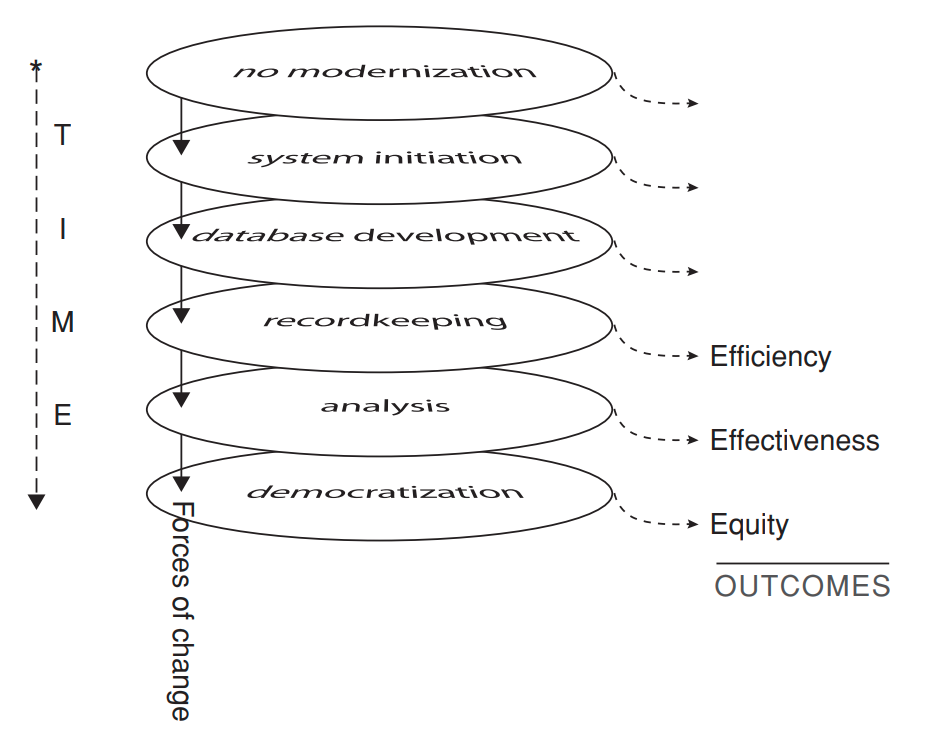
\includegraphics[scale=0.3]{Figures/chap2/gis_equity.png}
	\caption[Development of GIS development and associated outcomes]{Development of GIS development and associated outcomes. From \cite{tullochTheoreticalModelMultipurpose1999} as reprinted in \cite{tullochInstitutionalGeographicInformation2007}}
	\label{fig:gis_equity}
\end{figure}


One of the consequences of the Mumford-Winner view, however, is that it implies that the designers of technology have both agency and responsibility to determine what politics are embedded in their designs. To reject either the agency or the responsibility is highly problematic. Many designers of digital tools seek to reject the former and commit themselves to a sort of technological determinism \cite{sheppardGISSocietyResearch1995}. For example, Stephen Goldsmith and Susan Crawford, who did a great deal to implement such technologies in New York City and Indianapolis, wrote that "the process of collection is \textit{not going to stop}. We think, it fact, that it would be shortsighted and \textit{probably impossible to halt this natural evolution}. That is all the more reason, then, to carefully establish policies covering data access, data security, and transparency with respect to its collections" (emphasis mine) \cite{goldsmithResponsiveCityEngaging2014}. They thus divorce themselves of responsibility for the design of the technology itself and restrict themselves for seeking to govern who uses it.

Meanwhile Goodspeed writes about the opposite problem, "Planning theorists have too often accepted Habermas's view that technology is primarily associated with technical rather than moral rationality, which leads them to overlook technology's potential normative dimension... Even choosing a digital tool requires making value-laden judgments about what issues matter enough to be analyzed. Because digital tools typically inherit the worldviews and assumptions of their creators, even well-meaning applications of them can inhibit potentially valuable new ideas or critical perspectives." He then proposes the term \textit{tool of inquiry} to "describe the ideal in which tools are continually shaped, used, and tested by public users," \cite{goodspeedScenarioPlanningCities2020} thereby aligning it with the democratic, human-centered type of technology. As Monmonier noted, ``A single map is but one of an indefinitely large number of maps that might be produced for the same situation or from the same data." \cite{monmonierHowLieMaps1996} We must therefore thoughtfully consider how that single map is selected.

We must recognize that, as Krygier and Wood so playfully illustrated, maps (and all \acp{gis}) are, fundamentally, propositions about that world that are asserting a fact and promoting an action. Because of this "you must accept responsibility for the realities you create with maps" \cite{krygierCeEstPas2011}. And this is not limited to maps. Design itself is purposeful in that it forges both pathways and boundaries in its instrumental and cultural use" (\cite{paceyCultureTechnology1983} as paraphrased in \cite{nobleAlgorithmsOppressionHow2018}). 

And there are clear examples of geospatial data being using for positive impact. For instance, there is \ac{nasa}'s famous Blue Marble image, which, while perhaps more iconic than cartographic, is still undeniably a geospatial object, a map even, that has essentially created both "one-world" discourse and "whole-earth" discourse \cite{propenCartographicRepresentationConstruction2011}. If that seems to much of a reach or too incidental, we can look at how Laura Kurgan and others used their "Million Dollar Blocks" project to powerful visualize the impact of mass incarceration upon particular, primarily black, American communities, helping to shift public perception and policy discussions \cite{kurganCloseDistanceMapping2013}. Or how the Sierra Club has made significant use of Google Earth in their efforts to garner support for conservation efforts in the US Arctic National Wildlife Refuge and elsewhere \cite{propenCartographicRepresentationConstruction2011}. Florence Nightingale's famous rose diagrams famously shifted policy on the handling of sanitation in war zones \cite{friendlyBriefHistoryData2008}, even if these diagrams were, in fact, misleading (cite).

Additionally, in some ways, we want to avoid making a seamless tool, as "the most significant impacts of technology tend to occur when the technology becomes indistinguishable from the fabric of every day life" (\cite{weinerComputer21stCentury1991} as paraphrased in \cite{vereginComputerInnovationAdoption1994}). This is not, unfortunately, not sufficient. "We all tend to defer to machines, which can seem more neutral, more objective" even when they are actively warning us of their limitations and fallibility \cite{eubanksAutomatingInequalityHow2018}.

I do align myself with those who feel that:

\blockquote{Even though the funding or research and development... of GIS and other imaging systems has come primarily from business, state, and military sources, advocates of the progressive potential information and imaging technologies argue that access is hard to deny, networks are difficult to control, information is readily accessible and used by individuals and groups with limited budgets and expertise, and the ability to use the technology in depth permits groups like environmental organizations to counter claims by polluters about their environmental impacts, by developers about likely local effects of runoff and ground water, and so on... GIS enables communities to make better decisions by providing access to more and better information. It offers more powerful tools for local planning agencies; it offers exciting possibilities for data coordination, access, and exchange; and it permits more efficient allocation of resources, and a more open rational decision-making process} \cite{picklesRepresentationsElectronicAge1994}. 

That said, I don't believe that any of this is guaranteed or effortless. It requires intentionality and reflection on the part of the designers, as well as a humble willingness to listen to criticism from anyone, including those who are not `experts.' This was a key point of the various critical \ac{gis} movements discussed in Section \ref{sec:collaborative}. Their work is demonstration that it is possible develop and apply \ac{gis} in a collaborative and participatory manner.

As we proceed, we must keep in mind that "the very notion that technologies are neutral must be directly challenged as a misnomer," \cite{nobleAlgorithmsOppressionHow2018} and that, as Smithsonian curator Lucy Fellowes said, "Every map is someone's way of getting you to look at the world his or her way" \cite{henriksonPowerPoliticsMaps1994}. 

%"It is also not clear that geography's diversity is a flaw instead of a great strength. Geography is inherently eclectic because the discipline is defined only by a perspective on the world. However, those who advocate the computer as a means to unify geography have a particular conception of the discipline in mind, an empirical and pragmatic one that is by no means universally accepted." \cite{vereginComputerInnovationAdoption1994}


%"Mappings do not represent geographics of ideas; rather they effect actualization... Maps remake 'territory over and over again, each time with new and diverse consequences'" (\cite{cornerAgencyMappingSpeculation1999} as paraphrased by \cite{kitchinThinkingMaps2011}).


%"Those who have the power to design systems - classification or technical - hold the ability to prioritize hierarchical schemes that privilege certain tyeps of information over others." \cite{nobleAlgorithmsOppressionHow2018}

\subsubsection{\hlc[green]{Technocratic Planning \& International Development}} \label{sec:technocracy}

I should start off by noting that this section is not intended to consider all of the arguments for and against planning in general (for that see Klosterman \cite{klostermanArgumentsPlanning1985}), but instead to focus in on the narrower question of whether \textit{technocratic planning}, particularly in an international context, can be helpful and ethical. This is important because many \ac{evdt} applications are international or multinational projects, including both of those focused upon in this work.

By "technocracy" we mean the basic idea that "the human problem of urban design has a unique solution, which an expert can discover and execute. Deciding such technical matters by politics and bargaining would lead to the wrong solution" \cite{scottSeeingStateHow2020}. It is typical for a believer of this idea to quickly put themselves in the role of the "expert [who] can discover and execute." That said, they quickly find themselves beset by complexity and gapes in the data that frustrate their efforts. For such aspirants "legibility [is] a central problem," one that must be solved prior to addressing urban design itself. To this end, "exceptionally, complex, illegible, and local social practices" must be turned into "a standard grid whereby it [can] be centrally recorded and monitored." This, of course, requires immense simplification. These "state simplifications... have the character of maps. That is, they are designed to summarize precisely those aspects of a complex world that are of immediate interest to the mapmaker and to ignore the rest. To complain that a map lacks nuance and detail makes no sense unless it omits information necessary to its function." And the interest of these would-be-technocrats tends to be their "unique solution." Taken together, there are five specific characteristics of these simplifications \cite{scottSeeingStateHow2020}:

\begin{enumerate} \setlength{\itemsep}{0pt} \setlength{\parskip}{0pt} 
	\item{They are interested and utilitarian, aimed at a particular end.}
	\item{They are nearly always written, as opposed to visual or verbal.}
	\item{They are typically static and thus, perpetually out-of-date to at least some extent. "The cadastral map is very much like a still photograph of the current in a river."}
	\item{They are typically aggregate facts, not individual ones.}
	\item{They are standardized, so as to enable comparison and longitudinal analysis.}
\end{enumerate}

These individuals are what Easterly calls "Planners," to be distinguished by "Searchers," those who seek for bottom-up solution to specific, addressable needs \cite{easterlyWhiteManBurden2007a}. The Planners, meanwhile, fashion themselves into benevolent dictators (though they would eschew being called as such) focused on implementing their solution \cite{easterly2015}. Beyond outright failure, such endeavors have not infrequently caused immense social harms, including famines, cultural destruction, and environmental collapse. Furthermore, such technocratic planning is bound up in the history of colonialism and, while formal colonialism has ended, its impacts continue and certain mindsets are still embedded within such planning efforts \cite{sandercockCommentaryIndigenousPlanning2004}.

James Scott argued that four elements were necessary to precipitate the most tragic of social engineering disasters \cite{scottSeeingStateHow2020}:

\begin{enumerate} \setlength{\itemsep}{0pt} \setlength{\parskip}{0pt} 
	\item{The "administrative ordering of nature and society." This includes items like cadastral maps, surnames, census records, and a standardized legal system. As Theodore Porter put it, "Society must be remade before it can be the object of quantification." \cite{porter1992objectivity}}
	\item{A "high-modernist ideology," which Scott defines as a "strong," "muscle-bound" "self-confidence about scientific and technical progress, the expansion of production, the growing satisfaction of human needs, the master of nature... and the rational design of social order commensurate with the scientific understanding of natural laws."}
	\item{An authoritarian state that is both "willing and able" to wield power to enact the high-modernist ideology.}
	\item{A vulnerable civil society that "lacks the capacity to resist" the plans of that authoritarian state.}
\end{enumerate}

In essence what is "truly dangerous to us and our environment... is the \textit{combination} of the universalist pretensions of epistemic knowledge and authoritarian social engineering" \cite{scottSeeingStateHow2020}. Such a combination often takes the form of undue focus being places on specific metrics, with little interest in underlying causes and dynamics. "Many studies involve ranking places on one or more criteria, and allocating policy benefits accordingly. At its crudest this applied geography merely provides a list of winner and losers with no understanding of why the differences occur" \cite{taylorGeographicInformationSystems1994}.

With regard to the second element a key aspect is that, as Scott notes, high-modernist ideology is not scientific practice exactly. Rather, it is a "faith that borrowed from the legitimacy of science and technology." In fact, it was more an aesthetic predilection than anything scientific. Furthermore, the underlying ideas were in fact quite sympathetic. "Doctors and public-health engineers who did possess new knowledge that could save millions of lives were often thwarted by popular prejudices and entrenched political interests"  \cite{scottSeeingStateHow2020}. The dangers were when an authoritarian state adopted the aesthetic veilings of such ideas to justify actions, in the way that Social Darwinism used evolutionary theory to justify horrid actions. In this way "the classism and racism of elites are mathwashed, neutralized by technological mystification and data-based hocus-pocus." \cite{eubanksAutomatingInequalityHow2018} This ideology could also be considered a "dangerous form of magical thinking [that] often accompanies new technological developments, a curious assurance that a revolution in our tools inevitably wipes the slate of the past clean" \cite{eubanksAutomatingInequalityHow2018} (something that we are currently seeing repeated with discussions about Big Data and machine learning \cite{barnesBigDataSocial2014}).

The details lost in the necessary simplifications that the technocrat must make often turn out to not be so negligible after all. In the USSR, "a set of informal practices lying outside of the formal command economy - and often outside Soviet law as well - [arose] to circumvent some of the colossal waste and inefficiencies built into the system. Collectivized agriculture, in other words, never quite operated according to the hierarchical grid of production plans and procurements." \cite{scottSeeingStateHow2020} The technocratic leaders were often aware of this but so committed to their ideology that they had no alternative but to maintain a sort of pretense, which anthropologist Alexi Yurchak called `hypernormalization' \cite{yurchakEverythingWasForever2005}, that served to compound problems until the Soviet Union eventually collapsed. Such a phenomena is particularly visible in strictly planned capital cities that have, "as the inevitable accompaniment of [their] official structures, given rise to another, far more `disorderly' and complex city \textit{that makes the official city work} - that is virtually a condition of its existence" \cite{scottSeeingStateHow2020}.

Even the `successful' development projects often came at a high cost and raised the question of "successful for whom?" After all "Haussmann's Paris was, \textit{for those who are not expelled}, a far healthier city" (emphasis mine) \cite{scottSeeingStateHow2020}.

So, with all of this said, do we think that the field of planning still has a positive role to play in society? I will propose three arguments in favor of such an idea, none of which are wholly satisfactory, but together may amount to something credible.

First, we may attempt to avoid fulfilling the conditions proposed by Scott above. We may, for instance, refuse to do work in areas with authoritarian governments, though this would certainly neglect many in dire need. We may also reject the high modernist ideology in our planning. This is certainly easier, as I have been doing exactly that, but it should not be taken as trivial either. In many ways such an ideology is the default of the technologist, and it requires active self-reflection to avoid falling into that trap. 

And the unfortunate matter is, even if we assume that Scott is correct in that his conditions are the necessary and sufficient conditions, what are they conditions for? "The \textit{most tragic} episodes of state-initiated engineering" (emphasis mine) \cite{scottSeeingStateHow2020}. The egregiously racist influence that Robert Moses had the design of New York City \cite{winnerArtifactsHavePolitics1980} happened in at least somewhat democratic society, not an authoritarian one. While it did not directly lead to mass famine and death, it is hardly something that we would want to replicate. I daresay that we want to do more than avoid the most tragic outcomes and instead want to do active good. We must therefore look beyond merely avoiding Scott's conditions.

Second, we may argue that planning has simply "come a long way from focusing on single page map and a timescale of 20-30 years" \cite{robinsonSectionPlanFormulation1972}. It is certainly true that many of the tools have changed over the past few decades. Systems engineering, for instance, is a substantially different field than it was in the middle of the 20th century, as is discussed in Sections \ref{sec:se} and \ref{sec:se_critique}. Sachs meanwhile proposes that prescriptive economics should be modeled on clinical medicine and should not seek to attribute all negative outcomes to the same cause nor to prescribe the same solution to all problems, but instead to "make a differential diagnosis for the economic case at hand." He lays out several different conditions of poverty, for example, and proposes different solutions to each. Foreign aid is effective at treating the "poverty trap" condition (wherein "the country is too poor to make the basic investments it needs to escape from extreme material deprivation and get on the ladder of economic growth"), but less so for other conditions \cite{sachsAgeSustainableDevelopment2015}. In this way, he seeks to distance himself from the high modernist ideology, with its affinity for singular, simple solutions, while still doubling down on the technocratic approach in general. 

It should be noted, however, that Sachs has been a senior advisor to numerous states and the \ac{un} dating back to the mid 1980s and thus has had ample time to demonstrate his ideas. Nonetheless, many of the critiques referred to already were addressing this time period and some, such as Easterly \cite{easterlyWhiteManBurden2007a}, were specifically aimed at Sach's efforts, with some arguing that many of his projects left people worse off than before \cite{munkIdealistJeffreySachs2014}.

I do think that many of the methodological and technological changes over the past several decades are meaningful, but it also seems undeniable that these changes seem insufficient to ensure good outcomes. So we must look elsewhere for means of shoring up the deficiencies.

The third argument we may make that planning still has a positive role to play involves collaborative and participatory forms of planning, similarly to what was done for \ac{gis} \acp{dss} in Section \ref{sec:collaborative}. After all even one of the proponents of high modernist ideology recognized that "rational, hierarchical, closed-door decision strategies" had negative consequences and that "more democratic process might produces worse results, but it would respond to the increasing sense of alienation among the nation's urban population" \cite{lightWarfareWelfareDefense2005}. This avenue is not without its flaws, unfortunately. By providing tools for more participation, we are not necessarily changing anything fundamental. "Participation is not power; its reform is not radical" \cite{marcuseThreeHistoricCurrents2016}. Even if participation is quite extensive and includes actual political power, "democracies rarely end up expropriating and redistributing capital" \cite{fainsteinSpatialJusticePlanning2016}. Thus even "inclusive planning practices cannot 'shift the effects of (post)colonial structures and relations of power on indigenous nations without a fundamental recognition of rights'" \cite{sandercockCommentaryIndigenousPlanning2004}.

Not only is participation evidently insufficient on its own, but some argue that neoliberalism in factor prefers to use participation as a means of undermining resistance, rather than violence, though this has the risk of providing a structure for coalition building and radicalization \cite{miraftabInsurgentPlanningSituating2016}. This can occur even unintentionally, as "an inappropriate level of participation may disempower individuals... and it also can distract groups from a desired outcome" \cite{sieberPublicParticipationGeographic2006}. In fact, increased community involvement can result in more restrictive, unambitious goals that are not in the interests of certain minorities \cite{wheatonIdentifyingPublicInterest1972}. A key aspect of participatory planning is that mere participation does not magically eliminate power hierarchies. Such pre-existing hierarchies can wield their power in planning discussions in 
three primary ways: "by promoting formal decisions, setting the agenda, and influencing the broader ideological context of the debate" (\cite{foresterPlanningFacePower2001} as paraphrased by \cite{goodspeedScenarioPlanningCities2020}). Similarly, merely connecting individuals and enabling the sharing of information does not necessarily promote engaged political deliberation \cite{gordonAugmentedDeliberationMerging2011}.

Despite this, there is evidence that, with proper creation of the structures of participation or in the wholesale rejection of the state-led participatory structures, that planning can be used to promote equity and development. Goodspeed points out several examples of how participatory and even insurgent scenario-based planning helped address injustices such as racism in urban development \cite{goodspeedScenarioPlanningCities2020}. I discuss further evidence to this effect in Section \ref{sec:scenario_critique}.

To resolve this confusion, Arnstein rejects a the binary model of authoritarian vs participative and proposes an eight-step "ladder of civic participation," as seen in Figure \ref{fig:civic_ladder} \cite{arnsteinLadderCitizenParticipation1969}. In this model, there are different degrees of participation, with direct citizen control at the top to manipulation of the public by central authorities through means only nominally "participative" at the bottom (and the omitted zeroth step of direct central authority with no pretense of participation). In this vein, Bekkers and Moody provide some examples of visualization and \ac{gis} use that, while presented as efforts to inform and enfranchise the public, made the citizenry feel manipulated \cite{bekkersVisualEventsElectronic2011}. 

\begin{figure}[h]
	\centering
	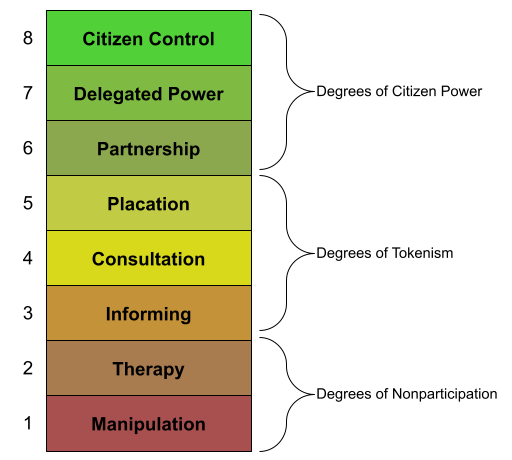
\includegraphics[scale=0.5]{Figures/chap2/civic_ladder.png}
	\caption[Arnstein's ladder of civic participation]{Arnstein's ladder of civic participation. Adapted from \cite{arnsteinLadderCitizenParticipation1969}.}
	\label{fig:civic_ladder}
\end{figure}

This suggests that, while technology-based collaborative or participatory planning efforts are unlikely to effect radical change, they can, \textit{if done well}, still affect positive change. Gordon and Manosevitch, building upon Gastil, argue that two components are needed to have truly participative planning: an 'analytic process' for sharing and analyzing information and a 'social process' for providing for deliberative discussion \cite{gordonAugmentedDeliberationMerging2011}. 

In line with some of Easterly's arguments, Virginia Eubanks proposers two gut check questions to ensure that a planning tool avoids harmful consequences \cite{eubanksAutomatingInequalityHow2018}:

\begin{enumerate} \setlength{\itemsep}{0pt} \setlength{\parskip}{0pt} 
	\item{Does the tool increase the self-determination and agency of the poor?}
	\item{Would the tool be tolerated if it was targeted at non-poor people?}
\end{enumerate}

Jonathan Furner, meanwhile, proposes three strategies for developing such tools (\cite{furner2007dewey} as paraphrased by \cite{nobleAlgorithmsOppressionHow2018}):

\begin{enumerate} \setlength{\itemsep}{0pt} \setlength{\parskip}{0pt} 
	\item{Admission on the part of designers that bias in classification schemes exists, and indeed is an inevitable result of the ways in which they are currently structured.}
	\item{Recognition that adherence to a policy of neutrality will contribute little to eradication of that bias and indeed can only extend its life.}
	\item{Construction, collection, and analysis of narrative expressions of the feelings, thoughts, and beliefs of classification-scheme users who identify with particularly racially-defined populations.}
\end{enumerate}

So, while I argue that a combination of new methodologies and technologies, collaborative and participatory design, and a general intellectual humility are sufficient to avoid the more harmful outcomes of the past (and present), Eubank's and Furner's points are worth keeping in mind as we continue.


%James Scott argued that "legibility [is] a central problem in statecraft." Through the act of making society and nature itself legible, "officials took exceptionally, complex, illegible, and local social practices... and created a standard grid whereby it could be centrally recorded and monitored. The organization of the natural world was no exception."  \cite{scottSeeingStateHow2020}


%Discuss and critique of informality as a concept \cite{royUrbanInformalityProduction2016}
%
%De Soto argues that the poor already have assets, just needs to be formalized. \cite{sotoMysteryCapitalWhy2003} though others argue that this is just results in a cycle of appeasment / welfare \cite{hollandForbearanceRedistributionPolitics2017}

\subsubsection{\hlc[green]{Systems Engineering}} \label{sec:se_critique}

So how does systems engineering relate to this discussion of technocratic planning? Well, systems engineering constituted one of the primary fields that technocrats drew upon, particularly in the 1950s-1970s. In 1964, the state of California commissioned four aerospace companies to conduct studies and develop models of the state's transportation needs for the coming decades \cite{smithSystemsApproachUrban1968}. US Vice President Herbert Humphrey said in a 1968 speech that ``The techniques that are going to put a man on the Moon are going to be exactly the techniques that we are going to need to clean up our cities" \cite{lightWarfareWelfareDefense2005}. In the same year, the RAND Corporation established the \ac{nycri} in an attempt to bring systems analysis and engineering to urban planning. Around the same time, the \ac{aiaa} hosted meetings on urban technologies to bring aerospace expertise to bear on the urban crises of the time \cite{lightWarfareWelfareDefense2005}. In 1970, NASA established the Urban Development Applications Project \cite{fosterUrbanDevelopmentApplications1970}, followed by a New York City Applications Project in 1972, and an NSF Urban Technology System Experiment in 1973 \cite{karenTechnologyTransferNew1973}. Also in 1970, Jay Forrester published his seminal paper ``Systems Analysis as a Tool for Urban Planning" \cite{forresterSystemsAnalysisTool1970} which in 1972 would be expanded upon with the World3 model used in the (in)famous book \textit{The Limits to Growth} \cite{meadowsLimitsGrowth1972}. System dynamics, the modeling approach underlying both of these, would go on to have major impacts on business management, urban development, and environmentalism \cite{forresterSystemDynamicsPersonal2007a}. The very same year, the US federal government established the \ac{usac} to bring systems engineering and analysis tools to municipalities across the country \cite{kraemerRequiemUSAC1979}. Outside of the US, the London-based think-tank, Centre for Environmental Studies, was advocating for the use of multiscale and multidomain urban models as early as 1968 \cite{wilsonModellingSystemsAnalysis1968}. It was a heady time, with engineers feeling ``that, having reached the moon, they could now turn their energies to solving the problem of growing violence in cities along with other urban ``crises" \cite{mazza2017}. These applications were justified by several different rationale, chief among them were \cite{lightWarfareWelfareDefense2005}: 

\begin{itemize} \setlength{\itemsep}{0pt} \setlength{\parskip}{0pt} 
	\item{Computer simulations and related techniques were simply advances on the statistical models already widely used by the urban planning profession.}
	\item{The rise of cybernetics, with its cross-disciplinary control analogies, promised to unify disparate fields within urban planning and analysis, resulting in a unified understanding of cities.}
	\item{The use of these military innovations would transform urban planning and decision-making into scientific endeavors.}
\end{itemize}

Almost immediately, however, such grand ideas met with difficulties. The \ac{nycri} was forced to close in 1975 in the face of resistance from the civil service, unions, and the public at large due to perceptions of RAND's elitism, secrecy, and lack of regard for the side effects of their proposed reforms \cite{lightWarfareWelfareDefense2005}. As early as 1972, RAND acknowledged that the \ac{nycri} attempt had met numerous difficulties due to such issues as the \ac{nycri}'s secrecy (the New York City council ``grew annoyed" that ``under the terms of our contracts [they have] no right of access to the studies" \cite{szantonAnalysisUrbanGovernment1972}) and \ac{nycri}'s failure to ``provide these groups [local interest groups] with the means of participating in public debate in a more informed and more rational way." \cite{szantonAnalysisUrbanGovernment1972} The \ac{usac} was shutdown in 1977 after significant criticism for spending large amounts of money on projects that failed to deliver \cite{kraemerRequiemUSAC1979}. NASA's efforts lasted somewhat longer, continuing to encourage the use of remote observation data by urban planners as late as 1980 \cite{rushRemoteSensingUtility1976, haggertySpinoff19801980} before retreating from the urban development domain in the early 1980s largely due to a lack of interest from municipal governments and planners \cite{lightWarfareWelfareDefense2005}. Perhaps the most ambitious application of systems engineering methodologies to economic development was the 1971-1973 Project Cybersyn, a distributed decision-support system based on an economic simulator and cybernetics intended to facilitate the management of Chile's national economy \cite{medinaCyberneticRevolutionariesTechnology2011}. Unfortunately Project Cybersyn is not particularly useful for understanding the benefits and limitations of systems engineering as it was abandoned following the nation's military coup in 1973, though even in prototype form it did yield some initial successes (and ran into various challenges) \cite{medinaDesigningFreedomRegulating2006}. 

Meanwhile, much of the US planning profession strongly rejected the new systems engineering entrants:

\begin{singlespcquote}
The systems engineers bring some expertise and substantial pretensions to the problems of the city. Their principal system expertise seems to be relative to complex organizations that are mission oriented. There is in any case a good deal of difference between the mission of reaching the moon, and the mission of survival and welfare for society and the city. The systems engineer can in general deal best with subsystems and specific tasks, and he therefore suboptimizes. This is a charitable description. \cite{robinsonDecisionmakingUrbanPlanning1972}
\end{singlespcquote}

\vspace{-7mm}

\begin{singlespcquote}
Trying to solve `earthly problems,' especially urban problems through aerospace innovations had shown that `transporting the astronauts from terra firma to land on the lunar sphere, travel hither and yon over its surface, and then back home to Houston' was a comparatively simple task. \cite{lightWarfareWelfareDefense2005}
\end{singlespcquote}

This perception continues to the present day. Figure \ref{fig:friedman_timeline} situates systems engineering and analysis among other intellectual schools of urban planning. It is positioned on the far left of the figure, indicating that the field "look[s] to the confirmation and reproduction of existing relationships of power in society. Expressing predominantly technical concerns, they proclaim a carefully nurtured stance of political neutrality. In reality, they address their work to those who are in power and see their primary mission as serving the state" \cite{mazza2017}. Marcuse, meanwhile, refers to systems engineering as primary concerned with efficiency and highly deferential to existing relations of power: "the technicist is inherently conservative: it is to serve an economic and social and political order in which its role is to make that order function smoothly." \cite{marcuseThreeHistoricCurrents2016}. It is natural that the more authoritarian-minded decision-makers would thus find systems engineering of interest. It was not only in dictatorships that systems engineering found a planning home, however. Many of the examples cited above where within the United States. In keeping with Scott's theory of social engineering disasters, the democratic nature of the US kept these applications from becoming large scale tragedies, but this does not mean they were successes by any means either. 

\clearpage
\begin{landscape}
\begin{figure}[t]
	\centering
	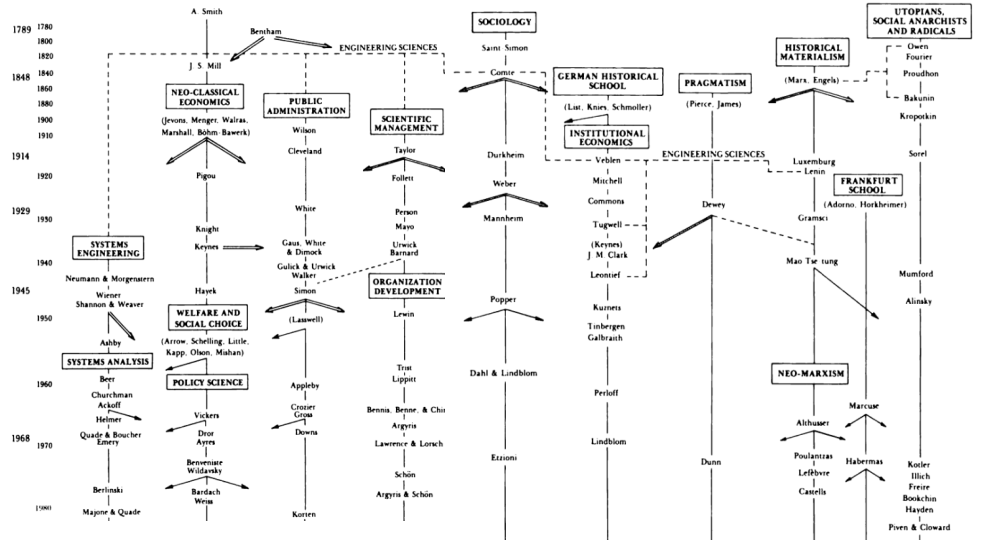
\includegraphics[scale=0.60]{Figures/chap2/friedman_timeline.png}
	\caption[Timeline of intellectual influences on American planning theory]{Timeline of intellectual influences on American planning theory. From \cite{mazza2017}}
	\label{fig:friedman_timeline}
\end{figure}
\end{landscape}
\clearpage

This part of the history of systems engineering is largely missing in most discussions within the field. Most start in the early 1950s and acknowledge that the field truly hit its stride with the Space Race of the late 50s and 60s \cite{gorodSystemofSystemsEngineeringManagement2008, bootonDevelopmentSystemsEngineering1984, hallHallMethodologySystems1962, brillSystemsEngineeringRetrospective1998}. The official formation of a professional society, the \ac{incose}, would follow much later in the early 90s \cite{honourINCOSEHistoryInternational1998}. These histories tend to focus on the technical development of the field, highlighting new methodologies and frameworks such as \ac{mbse}, \ac{sos}, etc.; or academic milestones, such as the formation of the IEEE Systems Journal or the promulgation of MIL-STD-499. The only consistently mentioned application of systems engineering is the Apollo program, though some of these histories occasionally mention other military or NASA programs such as \ac{tdrss}.

Typically lacking in these histories is discussion of notable application lessons learned, particularly from failures or shortcomings. Such a lack can lead to each new generation of engineers using new tools to replicate the mistakes of the past. This is not to say that the systems engineering field has wholly ignored failures. Talbott summarized systems engineering insights from several hundred system failures across several disciplines including aerospace engineering (e.g. the Hubble Telescope mirror defects), civil engineering (e.g. the Tacoma Narrows Bridge collapse), and telecoms (e.g. a worm on ARPAnet) \cite{talbottWhySystemsFail1993}. Bahill and Henderson conducted a similar review, though they also (unusually) included a couple of social systems, namely the US war in Vietnam and the failure of US counterintelligence to prevent the September 11th, 2001 terrorist attacks \cite{terrybahillRequirementsDevelopmentVerification2005}. Petroski has written extensively on lessons learned from civil engineering failures (primarily bridge and other structural collapses) that are generalizable to engineers of all disciplines \cite{petroskiEngineerHumanRole1992, petroskiDesignParadigmsCase1994}. A 2011 panel of senior practitioners in the field examined multiple aerospace failures from a systems engineering perspective \cite{slegersLearningFailureSystems2012}. 

These histories all omit the flawed use of systems engineering for urban planning during the middle of the 20th century. This gap, particularly striking when compared to the previously discussed histories of \ac{gis} and mapping, is highly concerning and lends weight to the critiques of systems engineering quoted above. To better respond to this, I conducted my own pair of reviews of the period, one systematic, focused on the systems engineering literature, and the other integrative, including sources from outside the systems engineering discipline. For full details on the methodology, see  \cite{reidSystemsEngineeringAppliedPendingPublication}. In this section, I present some of the results and discuss its relevance to the critique of technocracy and of systems engineering in particular.

Ultimately, across both the systematic review and the integrative review, eight pitfalls were identified (\textbf{P1-8}) which were then organized into three themes (\textbf{T1-3}). These, along with the portion of the reviews that noted each pitfall, are summarized in Table \ref{tab:pitfall_counts}. These pitfalls and themes are not the only possible way to categorize the pitfalls present across the literature, nor are they wholly independent from one another. These were selected and organized so as to facilitate useful lessons learned and actionable responses.

\newpage

\newgeometry{margin=3cm}

\begin{landscape}
\begin{table}[htbp]
\footnotesize
\caption[Identified Themes and Pitfalls from reviews, including the proportion of systematic and integrative review publications that contained each pitfall]{Identified Themes and Pitfalls from reviews, including the proportion of systematic and integrative review publications that contained each pitfall. From \cite{reidSystemsEngineeringAppliedPendingPublication}.}
\label{tab:pitfall_counts}
\begin{center}
\begin{tabular}{ C{3cm}   C{2cm}  L{11cm}  C{2cm}  C{2cm} } \hline
\textbf{Theme} & \textbf{ID} & \multicolumn{1}{c}{\textbf{Pitfall Description}}  & \textbf{Systematic Review} & \textbf{Integrative Review} \\ \hlinewd{2pt}
\multirow{2}{2cm}{\parbox{1\linewidth}{\vspace{0.5cm} \centering \textbf{T1}: Technical Limitations \& Simplifying Assumptions}} & \textbf{P1:} Data \& Metrics & Lack of relevant and low uncertainty data and indicators. This historically has been particularly severe in the case of social wellbeing. This lack of good metrics can result in optimizations based upon narrow metrics. &  60\% & 80\%\\ \cline{2-5}
& \textbf{P2:} Theory \& Methods & Lack of understanding, theory, or methodologies to handle the complexity of cities and societies. This can result in overly simplified models and the design of simple, controllable systems that do not work well in the field. & 43\% & 70\% \\ \hline
\multirow{4}{2cm}{\parbox{1\linewidth}{\vspace{2cm} \centering \textbf{T2}: Stakeholder \& Contextual Consideration}} & \textbf{P3:} Siloed Knowledge & Lack of integration across fields of research and other forms of knowledge. This can lead to a lack of regard for subject matter experts (e.g. urban planners, social scientists, etc.), historical context of intervention areas (i.e. assuming every city can be treated the same), and local expertise (e.g. long-term residents or community organizers). &  40\% & 80\% \\ \cline{2-5}
& \textbf{P4:} Singular Solution & The assumption that there is a single objective function to be optimized, that there is a singular `optimal solution', or that the needs of all stakeholders except the client can be safely ignored.  & 54\% & 50\% \\ \cline{2-5}
& \textbf{P5:} No User Focus & Lack of collaboration or interaction between the engineer/analyst and decisionmakers, system users, and/or the public. This can result in prioritization of basic research over the needs of the actual system stakeholders.  & 53\% & 90\%  \\ \cline{2-5}
& \textbf{P6:} Cost \& Time & Development of systems engineering analyses and tools either lagging the urgent need for a particular policy decision or being too costly to pursue and maintain.  & 9\% & 50\% \\ \hline
\multirow{2}{2cm}{\parbox{1\linewidth}{\vspace{0.5cm} \centering \textbf{T3}: Self-Awareness}} & \textbf{P7:} Lessons Learned & Lack of learning from past failures and experiences &  14\% & 50\% \\ \cline{2-5}
& \textbf{P8:} Hype & Overstating systems engineering capabilities or using engineering terminology to justify unscientific methods/actions. &  3\% & 30\% \\ \hline
\end{tabular}
\end{center}
\end{table}
\end{landscape}

\restoregeometry


\textbf{P1: Data \& Metrics} and \textbf{P2: Theory \& Methods} represent primarily technical limitations in data, metrics, and methodologies, coupled with the general intransigence of social systems to measurement and modeling. The first of these deals primarily with the much more limited and fuzzy data that systems engineers had to work with in planning contexts during the mid 20th century, as well as limited performance metrics for social wellbeing at both the individual and community scales. The latter refers to limitations in modeling methods and theoretical frameworks for grappling with the complicated dynamics of human societies. Such limitations encourage simplifying assumptions in order to make the problems tractable. One of the most common of these simplifications was selecting an efficiency metric for an existing system to optimize, rather than more critically considering the goals and design of the system as a whole \cite{mazza2017, marcuseThreeHistoricCurrents2016}. Both of the \textbf{T1} pitfalls were commonly identified in both reviews, likely because identification of technical limitations, along with proposals for how to address them, constitute a major mechanism for research progress. Beyond this, however, some issues, particularly around social questions, have no single, encompassing metric, regardless of the level of data availability. 

This directly leads into \textbf{T2}, which includes \textbf{P3: Siloed Knowledge}. As was discussed previously, planning literature abounds with complaints of systems engineers not considering disciplinary expertise or other forms of knowledge. Urban planners sometimes felt as though engineers sought to replace them rather than collaborate \cite{lightWarfareWelfareDefense2005}. Perhaps due to the data and computational limitations at the time, engineering models tended to focus on the abstract and universal, ignoring local context. Forrester's system dynamics model of a city, for instance, was critiqued for being ``not spatially disaggregated", ``of an abstract city", and for ``us[ing] no data" \cite{leejrRequiemLargeScaleModels1973}. \textbf{P4: Singular Solution}, regarding the extent to which a single objective function representing a single stakeholder's preferences is even appropriate, is an issue the systems engineers have had to grapple with even outside of planning contexts. This issue was recognized early on, though productive means of addressing were only developed much later. Smith in 1968 wrote that ``It is relatively easy to answer the question: `Who and what is missile XYZ being designed for?' It is significantly more difficult to answer the question: `For what users and what purposes is the city to be designed?'" \cite{smithSystemsApproachUrban1968} Similarly, Rider, in a 1975 \ac{nycri} paper demonstrating a parametric model for the allocation of fire companies, readily recognized that ``Far from involving the optimization of some well-defined criterion, the pursuit of such a goal requires the delicate integration of several often conflicting objectives... These questions have no universally acceptable solutions" \cite{riderParametricModelAllocation1975}.

Some of the notable differences between the systematic review and the integrative review are worth discussing. \textbf{P5: No User Focus} was mentioned in approximately half of the systematic review publications but almost all of the integrative review publications. Two primary causes of this pitfall were noted in the literature. The first is that many of the systems engineering applications were more focused on research, including developing and demonstrating new tools and techniques, rather than on responding to the immediate needs of decision-makers. The second was an emphasis on secrecy both towards decision-makers and the public at large. Both of these were likely disciplinary norms inherited from systems engineering's origins in military and private industry.

\textbf{P6: Cost \& Time}, which refers to higher than anticipated startup costs for systems engineering studies and models, was noted by only 9\% of publications in the systematic review but was noted in 50\% of the integrative review publications. This difference is likely due to two sources. First, scholarly research publications do not often complain about their own lack of funding or compressed deadlines, preferring to restrict themselves to technical results (with perhaps an appeal for future research support in the future). The second, noted in a number of publications found in both reviews, was a combination of general optimism with an expectation that tools and techniques developed in an aerospace or defense context could be directly ported over to urban and regional development with minimal additional resources. This ultimately proved to not be the case, and while both civilian and military aerospace projects could be assured of immense funding and institutional support during the Space Race era, these urban development applications often lacked such long term, invested support. Furthermore, if the development of a spacecraft was delayed, the launch date would be pushed back. In an policymaking setting, if the model development was delayed, a decision would simply be made without the model.

\textbf{P7: Lessons Learned} also has a significant gap between the systematic and integrative reviews. It should be noted that almost all of the publications included some amount of background or a review of the literature, as is to be expected. These typically focused on specific technical limitations of previous work that the new publication seeks to address. \textbf{P7} does not refer to this, but to a broader consideration of what impacts, positive or negative, that previous impacts had on decision-makers and public. Such consideration was infrequently found in the systematic review. 

Another noticeable difference is the least commonly noted pitfall, \textbf{P8: Hype}. This was only discussed once in the systematic review but was raised in several of the integrative review publications. This is perhaps because this is a critique that would rarely, if ever, be levied against one's own field. The systems engineering literature is populated by actual practitioners presenting primarily on their own results and thus, quite reasonably, believe in the validity and scientific merit of their own activities. Outside critics, however, are more prepared to identify hyperbole and deep methodological flaws. Forrester's system dynamics model of a city \cite{forresterUrbanDynamics1969} was criticized for ``bur[ying] what is a simplistic conception of the housing market in a somewhat obtuse model, along with some other irrelevant components. He then claims that the problem cannot be understood without the irrelevant complexity" \cite{leejrRequiemLargeScaleModels1973}. The one systematic review paper to discuss \textbf{P8} positioned itself as seeking to preserve the systems analysis / systems engineering field from ``overblown promotion" by ``opportunistic converts" who bring ``discredit to both the convert and his new-found meal ticket." \cite{brewerSystemsAnalysisUrban1973} Scott, meanwhile, pointed out that, regardless of the intellectual rigor of the underlying analysis, decisionmakers who commission a study can, through their influence of the study, direct its outcome in much the way that Forrester's model was accused. These decisionmakers can then drape themselves in the authority of a ``a scientific report" to justify their already decided upon course of action \cite{scottSeeingStateHow2020}. This is of course closely connected to stakeholder considerations posed by the \textbf{T2} pitfalls.


The frequency and content of publications in the literature records the gradual rejection and retreat of systems engineering from planning applications. As early as 1973, planning scholars were (perhaps preemptively) eulogizing the death of large-scale models and other tools of the systems engineer \cite{leejrRequiemLargeScaleModels1973}. The subsequent decades saw the fields of systems engineering and development planning grow largely independently of one another.

With regard to \textbf{P1: Data \& Metrics}, numerous quantitative economic and social indices have been developed for the planning field \cite{boyceFrameworkDefiningApplying1972, cliftonQuantitativeAnalysisUrban2008,readAssetbasedEconomicDevelopment2012,sawickiNeighborhoodIndicatorsReview1996,valRegionalLocalEconomic1991} and available data sources have greatly expanded, including telecoms-based mobility data, distributed sensors, remote observation, and demographic statistics. Mathematical tools such as cellular automata and agent-based modeling have become popular \cite{battyCitiesComplexity2005,laufUncoveringLanduseDynamics2012}. Digital models underlie the popular subdiscipline of scenario planning \cite{goodspeedScenarioPlanningCities2020,zapataRadicalUncertaintyScenario2015}. Interdisciplinary, integrated models have even started to re-emerge \cite{millerIntegratedUrbanModeling2018,moeckelTrendsIntegratedLanduse2018,shahumyanIntegrationLandUse2017}. 

At the same time, systems engineering has changed.  As early as 1981, systems engineers were incorporating some of the more critical perspectives into their work, as seen in \ac{ssm} which sought to shift emphasis from directly engineering social systems to leveraging a systems perspective during a process of inquiry \cite{checklandSystemsThinkingSystems1999}. In general, the belief that systems, even human systems, can be made simple, rational, and controllable (\textbf{P2: Theory \& Methods}) has been largely outmoded. Instead, systems engineers have adopted theories of complex systems. This change puts systems engineers in line with critical development planner Jane Jacobs, who argued that ``intricate minglings of different uses are not a form of chaos. On the contrary they represent a complex and highly developed form of order" \cite{jacobsDeathLifeGreat2016}. Complex systems, emergence, ``ilities", systems-of-systems, and complex adaptive systems have all become popular fields of study within systems engineering \cite{mcdermidComplexityConceptCauses2000, sussmanCollectedViewsComplexity2002, chenComplexityEmergenceEngineering2009, deguetElementsEmergenceIssue2006, officeofthedirectorofsystemsandsoftwareengineeringSystemsEngineeringGuide2008, glassComplexAdaptiveSystems2011, incosecomplexsystemsworkinggroupComplexityPrimerSystems2016, keatingSystemsSystemsEngineering2011, mittalHumanLoopSystem2015, sheardPracticalApplicationsComplexity2005, tolkResearchAgendaSupport2015}, with numerous frameworks being proposed for how to classify and handle such systems \cite{kurtzNewDynamicsStrategy2003, martinFrameworkQuantifyingComplexity2004, sheardComplexityTypologySystems2010, righiCharacterizingComplexitySociotechnical2012, schottlQuantifyingComplexitySocioTechnical2015, reymondetFrameworkSenseMakingComplex2016}. Faced with such systems, engineers have had to recognize their own inability to definitively predict the future and have turned to probabilistic and flexible methods that instead ``manage" complexity over longer time scales, such as epoch-era analysis \cite{rossUsingNaturalValueCentric2008, vascikMethodExploringProgram2015} (which has many similarities to the aforementioned urban planning method called scenario planning) and fuzzy probabilistic programming \cite{zhangRobustStochasticFuzzy2009, liuInexactStochasticFuzzy2015}. This can be seen in a recent set of definitions promulgated by \ac{incose}, which includes terms such as ``transdisciplinary," ``integrative," ``socio-technical systems," and ``complex systems," as well as a recognition that systems are conceptual abstractions with a chosen focus \cite{sillittoSystemsEngineeringSystem2019}. 

Parallel to this, systems engineers have moved away from narrowly implementing the directives and priorities of an individual client (\textbf{P4: Singular Solution} \& \textbf{P5: No User Focus}) to identifying, mapping, and analyzing the various stakeholders in a system in order to inform the architecture of the system and its requirements. Stakeholder analyses can involve both qualitative and quantitative tools, such as the Stakeholder Requirements Definition Process \cite{incoseINCOSESystemsEngineering2015}, Stakeholder Value Network Analysis \cite{fengDependencyStructureMatrix2010a}, and interviews of representatives from different stakeholder groups. This change in focus can also be seen in the rise of human-centered and user-centered design perspectives, which have spawned numerous specific methodologies and seen application in healthcare \cite{samarasSystemsEngineeringPerspective2005}, Industry 5.0 \cite{longoValueOrientedEthicalTechnology2020}, \ac{mbse} \cite{kimChallengesApplyingModelbased2019}, and other fields \cite{ritterFoundationsDesigningUserCentered2014}.

Such changes also serve to address \textbf{P3: Siloed Knowledge} by accepting information from a wider range of disciplinary sources and methods. In order to translate these complicated networks of stakeholders into designs, systems engineers have developed methods for handling multi-stakeholder negotiation and \cite{fitzgeraldEffectsEnhancedMultiparty2015,fitzgeraldRecommendationsFramingMultistakeholder2016,weckMULTISTAKEHOLDERSIMULATIONGAMING2012} tradespace visualization and exploration \cite{fitzgeraldEffectsEnhancedMultiparty2015,fitzgeraldRecommendationsFramingMultistakeholder2016,groganInteractiveModelsSystem2015,rossMultiAttributeTradespaceExploration2004,selvavaleroRulebasedSystemArchitecting2012}, the latter of which demonstrates an increased willingness to appreciate the psychology and experience of the user. Multiple of these techniques can even be linked together, such as when Sparrevik et al. combined participatory stakeholder engagement with multicriteria decision analysis for the management of a harbor, emphasizing the lateral learning and trust that can develop through such a transparent process \cite{sparrevikUseMulticriteriaInvolvement2011}. Such techniques can thus been seen as a response to a common historical critique that systems engineers assume ``complex controversies can be solved by getting correct information where it needs to go as efficiently as possible," that ``political conflict arises primarily from a lack of information," and that ``if we just gather lack the facts... the correct answers to intractable policy problems like homelessness will be simple, uncontroversial, and widely shared" \cite{eubanksAutomatingInequalityHow2018}. Systems engineering thus has potentially useful tools and perspectives to contribute to the such endeavors as collaborative planning theory \cite{goodspeedDeathLifeCollaborative2016} and participatory development \cite{pertParticipatoryDevelopmentNew2013}.

With regards to \textbf{P6: Cost \& Time}, significant infrastructure has been put in place to support the urban planning profession. Interactive \acp{dss} abound \cite{waddellUrbanSimModelingUrban2002, walkerPlannersGuideCommunityViz2017}. The use of \ac{gis} has become the norm \cite{jankowskiGISGroupDecision2001,tomlinGISCartographicModeling2012,wilsonHandbookGeographicInformation2007}, including more participatory variants \cite{sieberPublicParticipationGeographic2006}. Systems engineering likewise has seen a heightened emphasis on re-usable tools and infrastructure in the form of both specific modeling languages like \ac{opm} \cite{doriObjectProcessMethodologyHolistic2002} and in general approaches such as \ac{mbse} \cite{ramosModelBasedSystemsEngineering2012}. Beyond planning and systems engineering, computational power has increased by orders of magnitude (which has then found use in new simulation techniques) and the public in general has become much more familiar with computational tools. All of these together have supplied the basic analysis infrastructure that is common to the field. As a result, new applications do not necessarily require immense resources.


These developments are summarized in Table \ref{tab:new_developments}. Taken together, they suggest that the fields of systems engineering and planning are perhaps closer to each other than ever before, even showing some elements of convergent evolution. This can be seen in the use of the term complex adaptive system in both fields \cite{yamuAssumingItAll2016}, as well as in the rise of industrial ecology \cite{chertowIndustrialEcologyDeveloping2008}. This latter field is bringing insights from systems engineering (among other fields) to bear on cities and the environment once more. Examples include thermodynamics and entropy modeling \cite{bristowWhyCitiesGrow2015, purvisThermodynamicEntropyIndicator2017}, metabolism \cite{kennedyStudyUrbanMetabolism2011}, and scaling laws \cite{loboUrbanScalingProduction2013}. Some of this work is explicitly picking up avenues of research from the 1970s that were abandoned in the 1980s \cite{kennedyStudyUrbanMetabolism2011}. Furthermore, many of the pitfalls from half a century ago identified by this paper have been significantly addressed in the literature. Much benefit could be gained through more direct dialogue and collaboration between systems engineering and planners. At the same time, none of these pitfalls have been wholly obviated, none of the new developments have achieved universal adoption, and the dangers of \textbf{P8: Hype} are always present, regardless of methodology. Some of the methods for addressing these pitfalls are in tension with one another. For example, the new modeling techniques aimed at addressing \textbf{P2} can increase opacity and inexplicability, thereby inhibiting the ability to involve decision-makers and the public in their development and build trust in its results (\textbf{P5}). 

So how can we make use of the opportunity for constructive collaboration, avoid falling prey to the same pitfalls as the past, and navigate these inter-pitfall tensions?

\newgeometry{margin=3cm}

\begin{landscape}
\begin{table}[H]
\footnotesize
\caption[New Developments for the Identified Pitfalls]{New Developments for the Identified Pitfalls. From \cite{reidSystemsEngineeringAppliedPendingPublication}.}
\label{tab:new_developments}
\begin{center}
\begin{tabular}{ C{3cm}   C{2cm}  L{8cm} C{5cm} } \hline

\textbf{Theme} & \textbf{Pitfall} & \multicolumn{1}{c}{\textbf{New Developments}} & \textbf{Relevant Publications}  \\ \hlinewd{2pt}

\multirow{2}{3cm}{\centering \textbf{T1}: Technical Limitations \& Simplifying Assumptions} & \textbf{P1} & Improvements in in-situ data collection (e.g. telecoms, distributed sensors, statistical agencies) and remote observation; new indices of societal and personal wellbeing & \cite{boyceFrameworkDefiningApplying1972, cliftonQuantitativeAnalysisUrban2008,readAssetbasedEconomicDevelopment2012,sawickiNeighborhoodIndicatorsReview1996,valRegionalLocalEconomic1991}  \\ \cline{2-4}

& \textbf{P2} & Complex systems, biomimicry, emergence, systems-of-systems, complex adaptive systems, epoch-era analysis, fuzzy probabilistic programming, agent-based modeling & \cite{battyCitiesComplexity2005,laufUncoveringLanduseDynamics2012, goodspeedScenarioPlanningCities2020,zapataRadicalUncertaintyScenario2015, millerIntegratedUrbanModeling2018,moeckelTrendsIntegratedLanduse2018,shahumyanIntegrationLandUse2017, checklandSystemsThinkingSystems1999, mcdermidComplexityConceptCauses2000, sussmanCollectedViewsComplexity2002, chenComplexityEmergenceEngineering2009, deguetElementsEmergenceIssue2006, officeofthedirectorofsystemsandsoftwareengineeringSystemsEngineeringGuide2008, glassComplexAdaptiveSystems2011, incosecomplexsystemsworkinggroupComplexityPrimerSystems2016, keatingSystemsSystemsEngineering2011, mittalHumanLoopSystem2015, sheardPracticalApplicationsComplexity2005, tolkResearchAgendaSupport2015, rossUsingNaturalValueCentric2008, vascikMethodExploringProgram2015, zhangRobustStochasticFuzzy2009, liuInexactStochasticFuzzy2015} \\ \hline

\multirow{4}{3cm}{\parbox{1\linewidth}{\vspace{1.5cm} \centering \textbf{T2}: Stakeholder \& Contextual Consideration}} & \textbf{P3} &  Stakeholder Value Network Analysis, qualitative interviews for use in requirement definition; general expansion of interdisciplinary teams & \cite{checklandSoftSystemsMethodology2000, fengDependencyStructureMatrix2010a} \\ \cline{2-4}

& \textbf{P4} &  Multi-attribute and multi-objective optimization methods; multi-stakeholder negotiation, tradespace visualization and exploration & \cite{fitzgeraldEffectsEnhancedMultiparty2015,fitzgeraldRecommendationsFramingMultistakeholder2016,weckMULTISTAKEHOLDERSIMULATIONGAMING2012, groganInteractiveModelsSystem2015,rossMultiAttributeTradespaceExploration2004,selvavaleroRulebasedSystemArchitecting2012}\\ \cline{2-4}

& \textbf{P5} &  Stakeholder Requirements Definition Process; Human-centered and user-centered design perspectives; open source software; end of the Cold War; increased role of non-military stakeholders in systems engineering discipline & \cite{incoseINCOSESystemsEngineering2015, goodspeedDeathLifeCollaborative2016, pertParticipatoryDevelopmentNew2013, samarasSystemsEngineeringPerspective2005, longoValueOrientedEthicalTechnology2020, kimChallengesApplyingModelbased2019, ritterFoundationsDesigningUserCentered2014} \\ \cline{2-4}

& \textbf{P6} & Advances in computing power; Decreases in computational cost; Increased public familiarity with computational tools; Development of re-usable tools and infrastructure (OPM, MBSE, etc.); independent development of urban planning models & \cite{waddellUrbanSimModelingUrban2002, walkerPlannersGuideCommunityViz2017, doriObjectProcessMethodologyHolistic2002, ramosModelBasedSystemsEngineering2012}\\ \hline

\textbf{T3}: Lessons Learned & \textbf{P7} &  Better histories of the field\\ \hline

\textbf{T4}: Hype & \textbf{P8} & \\ \hline
\end{tabular}
\end{center}
\end{table}
\end{landscape}
 
\restoregeometry

I propose three tactics for collaboration between the fields of systems engineering and planning:

\begin{enumerate} \setlength{\itemsep}{0pt} \setlength{\parskip}{0pt} 
	\item{Adopt the new developments that address certain historical pitfalls (as summarized in Table 4) and continue to pursue new opportunities to address the remaining dangers.}
	\item{Explicitly grapple with the history of systems engineering in planning. Use this to expand the sphere of collaboration.}
	\item{Select an application domain that can benefit greatly from both systems engineering and planning, preferably a relatively novel domain, then put together multidisciplinary teams to address that domain.}
\end{enumerate}

The first is straightforward. As has been discussed, fifty years ago, systems engineering lacked the disciplinary tools and perspectives necessary to successfully tackle many areas within planning. While significant gaps remain, new methodological developments in both fields mean a new opportunity for collaboration.

The second is necessary to avoid new generations of systems engineers being educated in ignorance of past mistakes. None of the pitfalls listed in Table 4 were based entirely on technical shortcomings and most were primarily nontechnical in origin. Many had to do with perspective and personal approach, often characterized by a certain disciplinary hubris. The urban planners of the 1970s felt that systems engineers wanted to replace them, rather than collaborate with them. Much of the public felt that the systems engineers were the servants of entrenched powers rather than the community at large. Regardless of the truth of these perceptions, their mere presence significantly hampers the ability of systems engineers to effectively implement their projects. Both can be addressed via a certain professional humility and a willingness to engage in true multi-stakeholder decision-making. In many ways this is an extension of an already present norm within systems engineering. From its beginnings, systems engineers have depended upon multidisciplinary teams of engineers. After all, systems engineers are largely unnecessary for projects that can be accomplished by a single engineer and for a single stakeholder. Teamwork, communication, and collaboration are thus fundamental to the field. Over time, the boundaries of these collaborations expanded to include multiple organizational stakeholders in a single project, including multiple clients, government agencies, and non-client beneficiaries. What we are now proposing is to expand this still further, by including both technical experts such as environmental scientists, ecosystem services economists, and anthropologists; and nontechnical members of the communities in which our systems operate. Such a proposal has been previously advanced, particularly with regard to the inclusion of social scientists, in the form of emphasizing the importance of the ``ologies" \cite{donaldsonPraiseOlogiesDiscussion2017}. Beyond this however, we are arguing for a participatory systems engineering, taking a page from the fields of \ac{gis} and planning that have been building participatory frameworks and tools for the past couple decades \cite{kimCriticalCartographyParticipatory2015,
pertParticipatoryDevelopmentNew2013,
sieberPublicParticipationGeographic2006,
talenBottomUpGIS2000,
ulibarriCollaborativeModelDevelopment2018}. This is also in line with the field of remote sensing, which has a similar Space Race military origin and has recently seen a more participative research agenda mapped out \cite{bennettPoliticsPixelsReview2022} (as discussed in Section \ref{sec:remote}). Systems engineering already has many of the tools for this, in the form of multi-stakeholder negotiation methods and tradespace exploration tools. These can be readily adapted to to incorporate community perspectives and be used as part of existing collaborative scenario planning processes common in urban planning.

The third approach is appropriate not only because it allows for plenty of research opportunities, but it avoids one field (systems engineering or planning) dominating the other due to historical entrenchment. Urban planner Scott Campbell recognized a similar need within his own field \cite{campbellGreenCitiesGrowing2016}:

\blockquote{The danger of translation is that one language will dominate the debate and thus define the terms of the solution. It is essential to exert equal effort to translate in each direction, to prevent one linguistic culture from dominating the other... Another lesson from the neocolonial linguistic experience is that it is crucial for each social group to express itself in its own language before any translation. The challenge for planners is to write the best translations among the languages of the economic, the ecological, and the social views, and to avoid a quasi-colonial dominance by the economic \textit{lingua franca}, by creating equal two-way translations... Translation can thus be a powerful planner's skill, and interdisciplinary planning education already provides some multiculturalism.}

The question then, is what domain would be fruitful for this endeavor? Campbell suggests that ``the idea of sustainability lends itself nicely to the meeting on common ground of competing value systems." As should be obvious at this point, I tend to agree with him, while noting that just because sustainable development is an apt proving ground, it does not mean that it is the only domain well suited for such collaboration.

\subsection{\hlc[green]{Sustainable Development \& the SDGs}} \label{sec:sdg_critique}

The concept of sustainable development as espoused by \acp{ngo} and UN agencies is not without critique. Nor is the specific substantiation of sustainable development in the \acp{sdg}. There are three primary such critiques that this section will address:

\begin{enumerate} \setlength{\itemsep}{0pt} \setlength{\parskip}{0pt}
	\item Sustainable development has become essentially toothless. It is used primarily for greenwashing and providing cover for actions that would have been taken anyways, rather than motivating real change.
	\item The reliance on detailed, specific metrics such as the \ac{sdg} indicators not only distracts from the more important, though harder to quantify, goals of human and environmental wellbeing, but actually works against them. 
	\item Lack of data and unreliability of data inhibits our ability to meaningfully evaluate our progress towards metrics at all.
\end{enumerate}

All three of these are genuine concern that have some, not insignificant degrees of truth. I will briefly lay out each of this concerns before considering how they jointly impact the manner in which the work envisioned in this thesis should proceed.

The first critique is particularly concerning as the \acp{sdg} greatly increased the number of domains of interest compared to the \acp{mdg}. Where the \acp{mdg} included three issues of human health (child mortality, maternal health, HIV/AIDS, malaria, and and tuberculosis), the acp{sdg} include at least (child mortality, maternal mortality, tuberculosis, malaria, Hepatitis B, neglected tropical diseases, suicide, various non-communicable diseases, substance abuse, road injuries, reproductive care, hazardous chemical and pollution exposure, tobacco use, and more). While on one hand this is a proper recognition of the long list of items that contribute to a sustainable world, it does run the risk of diluting the importance of any particular issue or allowing organizations to cherry pick the issues that they were already interested in, particularly as the \acp{sdg} have no built in mechanism for prioritizing on goal, target, or indicator over another.  

As Campbell wrote \cite{campbellGreenCitiesGrowing2016}:

\blockquote{The pessimistic thought is that sustainable development has been stripped of its transformative power and reduced to its lowest common denominator. After all, if both the World Bank and radical ecologists now believe in sustainability, the concept can have no teeth: it is so malleable as to mean many things to many people without requiring commitment to any specific policies.}

Boosters of global goal setting argue that they provide a host of benefits including: 

\begin{itemize} \setlength{\itemsep}{0pt} \setlength{\parskip}{0pt}%
	\item{Global goals are critical for social mobilization and coordinated orientation.}
	\item{Global goals provide global peer pressure for adoption, monitoring, and action.}
	\item{Global goals mobilizing epistemic communities (experts, researchers, etc. These in turn can help map pathways to achieving the goals, making them seem more manageable and less remote.)}
	\item{Global goals mobilize stakeholder networks and thereby leverage capital and other resources.}
\end{itemize}

Sachs, for example, argues that "\ac{mdg} goal setting has energized civil society and helped to orient governments that otherwise might have neglected the challenges of extreme poverty... the \acp{mdg} have been important in encouraging governments, experts, and civil society to undertake the `differential diagnoses' necessary to overcome remaining obstacles" \cite{sachsAgeSustainableDevelopment2015}. Part of this difference of opinion is based on whether one views the individual components of sustainable development mutually reinforcing or as competitive for scant resources. Sachs is certainly in the former camp, as is the concept underlying Figure \ref{fig:services_wellbeing} earlier in this thesis. The latter camp can be seen embodied in Figure \ref{fig:sustainable_triangle}, which conceives of sustainable development as a balance of three conflicts. This is a view that Sachs criticized as "much too pessimistic... Investing in fairness may also be investing in efficiency, and... attention to sustainability can be more fair and more efficient at the same time." Despite this, he elsewhere admits the impact of the \acp{mdg} was uneven, with public health receiving the most attention, while sanitation and education were largely sidelined. \cite{sachsAgeSustainableDevelopment2015}


\begin{figure}[h]
	\centering
	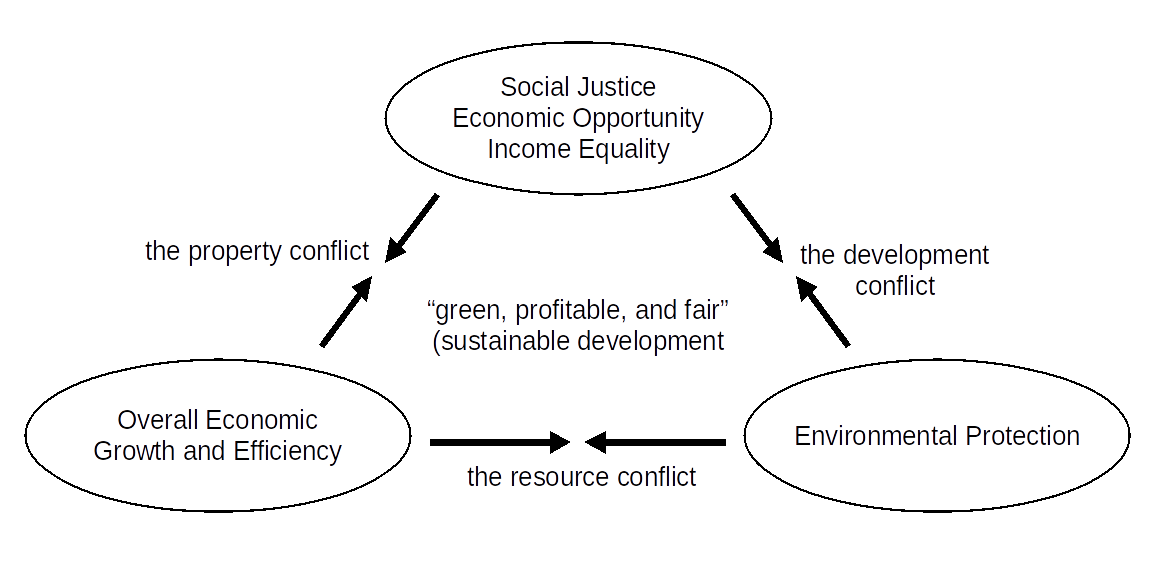
\includegraphics[scale=0.35]{Figures/chap2/sustainable_triangle.png}
	\caption[The triangle of conflicting goals of sustainable development]{The triangle of conflicting goals of sustainable development. Adapted from \cite{campbellGreenCitiesGrowing2016}}
	\label{fig:sustainable_triangle}
\end{figure}

Fukuda-Parr et al. advance this concern still further, pointing to evidence that the \acp{mdg} did little to raise awareness and motivate action for neglected priorities, but instead merely provided metrics for already popular initiatives \cite{fukuda-parrPowerNumbersCritical2014}. We must recognize that ability for global goals to motivate additional action by states and other actors is unclear. It is entirely possible that the creation of the \acp{sdg} primarily represents an increased interest by society at large in the idea of sustainability, rather than constituting a motivator for increased action itself. Even if this is the case, however, we can take some solace in the fact that idea of sustainability ``has become hegemonic, an accepted meta-narrative, a given. It has shifted from being a variable to being the parameter of the debate, almost certain to be integrated into any future scenario of development" \cite{campbellGreenCitiesGrowing2016}. The \acp{sdg} have become a kind of \textit{linga franca} when it comes to development projects and there is some utility in that. They can enable a certain shortcutting of having to explain why helping mangroves benefits society at large. Instead we can just point to \ac{sdg} Target 15.1.

Moving onto Critique 2, Fukuda-Parr et al. also pointed out that those issues that did see awareness raised and resources provided due to the \acp{mdg} produced "ambiguous impacts on complex social issues," particularly because some of the metrics were chosen for ease of implementation rather than importance. The primary strengths of the \acp{mdg} - "simplicity, mensurability, and concreteness - also proved to be sources of distortion" \cite{fukuda-parrPowerNumbersCritical2014}. Section \ref{sec:elitism} already partially addressed the more general sense of this problem, the concern that ``Substantive goals, the achievement of which are hard to measure, may be supplanted by thin, notional statistics - the number of villages formed, the number of acres plowed" \cite{scottSeeingStateHow2020}. Here I want to focus in one aspect that applied to the \acp{mdg} and \acp{sdg} in particular. 
 
One major critique of the \acp{mdg} was that they neglected human rights among their metrics, potentially justifying horrendous behavior by state actors and others as long as it made some number go up or go down as needed \cite{alstonShipsPassingNight2005}. This concern was even raised by the \ac{un} themselves in a public report towards the end of the \ac{mdg} lifecycle \cite{officeoftheunitednationshighcommissionerforhumanrightsWhoWillBe2013}. One obvious solution to this just incorporate human rights into the next round of goals, which is exactly what happened in \ac{sdg} 16, which numerous human rights issues from human trafficking to representative decision-making by governments. This likely also explains other, non-human rights additions to the \acp{sdg} as well.

This does not wholly address the issue of human rights (or other similarly neglected aspects or a holistic concept of development). Where under the \acp{mdg}, a decision-maker could say, ``Human rights aren't the list of goals, so they will take a backseat to Goal X," now under the \acp{sdg} they could simply say, ``We recognize that human rights are an important part of Goal 17, but we believe that Goal Y is more important for our nation (or some other nation in the case of an \ac{ngo})." Obviously many of the goods envisioned in the \acp{sdg} resist direct comparison or conversion to monetary terms, making it difficult to direct rebut such an argument. Even if you can justify some monetary conversion, Reddy and Heuty point out that any \textit{a priori} means of allocating priorities between goals on a cost-benefit basis is bound to fail due to the lack of data and highly unreliable approaches for estimating said costs and benefits \cite{reddyGlobalDevelopmentGoals2008}.

This leads directly in Critique 3. The uneven availability of data severely hampered international, expert-led development efforts, such as the \acp{mdg}. One of the more prominent of \acp{mdg} was Goal 6, ``Combat HIV/AIDS, malaria, and other diseases," with its associated Target 8: ``Have halted by 2015, and begun to reverse the incidence of malaria and other major diseases" \cite{inter-agencyandexpertgrouponmdgindicatorsMillenniumDevelopmentGoals2015}. It is difficult to measure progress towards this goal when, in 2005, some researchers indicated that that episodes of malaria globally may have been as much as 50\% higher than those reported by the \ac{who} \cite{snowGlobalDistributionClinical2005}. The availability and quality of data (commonly referred to as `monitoring') was thus a common element of critiques of the \acp{mdg} \cite{alstonShipsPassingNight2005,fukuda-parrPowerNumbersCritical2014,reddyGlobalDevelopmentGoals2008}. While many of these critiques used this as an argument for different fundamental models of international development that were not as data-reliant, proponents of the goals instead viewed this as a specific challenge to be overcome. As the \acp{mdg} were concluded and their successors, the \acp{sdg}, were created, the World Bank labeled the lack of a data a ``deprivation" on par with the lack of food, shelter, or healthcare \cite{DataDeprivationAnother}. The United Nations General Assembly, in its commissioning of the \acp{sdg}, ``called upon the United Nations system, including the Statistics Division of the Department of Economic and Social Affairs of the Secretariat and the regional commissions and international agencies, to support national efforts in building and strengthening national statistical capacity, in particular that of developing countries, and called upon all international agencies to improve the coverage, transparency and reporting on all indicators."

As was discussed in Section \ref{sec:remote}, remote \ac{eo} has been touted as globalizing data collection and addressing the data gap when it comes to the \acp{sdg}. Organizations such as \ac{geo} have even organized an initiative called EO4SDG to advance such activities \cite{grouponearthobservationsStrategicImplementationPlan}. Unfortunately, the historical rule that ``the poorer the country, the less and the worse the data" does not just apply to basic demographic and geographical data, such as that collected by standard decennial censuses or by national mapping services, but it also applies to data derived by analysis \cite{taylor1993full}, including global and multi-regional datasets. This is only exacerbated by the fact that such derived datasets are typically created by individuals and organizations based in the wealthier states and thus subject to their particular interests and language limitations. An example of this can be seen in the primary composite dataset of ecosystem services valuations. The \ac{esvd} is maintained by research organizations based in continental Europe and is primarily funded by a UK government agency \cite{grootEcosystemServicesValuation2020}. The database organizes the studies that it references by the location of the specific ecosystem services being valued. Table \ref{tab:esvd} shows the breakdown of the target continents of these studies, in which a bias can be seen both towards wealthier regions and towards those regions of more interest to the researchers and funding sources.

\begin{table}[H]
\caption[Regions studied by publications compiled by ESVD]{Regions studied by publications compiled by ESVD}
\label{tab:esvd}
\begin{center}
\begin{tabular}{ |C{4cm} | C{4cm} | C{4cm}| } \hline
\textbf{Region} & \textbf{Number of Studies} & \textbf{Percent of studies} \\ \hline
Africa & 309 & 7.7 \\ \hline
Asia & 1140 & 28.4 \\ \hline
Europe & 1639 & 40.8 \\ \hline
North America & 594 & 14.8 \\ \hline
Oceania & 223 & 5.6 \\ \hline
South America & 109 & 2.7 \\ \hline

\end{tabular}
\end{center}
\end{table}

This trend tends to be exacerbated in smaller sub-disciplines. Approximately 63\% of studies of mangrove-related ecosystem services are focused on parts of Asia despite these regions constituting providing only 38\% of the world’s mangrove coverage \cite{veghMangroveEcosystemServices2014}.

So how should this work be approached to avoid, or at least mitigate these critiques. First and most obviously, we can be careful about our collection and use of data so as to avoid technical mistakes. This includes such actions as characterizing gaps in the data rather than assuming them to be uniformly random, examining the generation process so as to identify potential errors, and not applying a data-based model out of its domain of calibration. In machine learning of remote observation data, for example, training data should typically be based on in-situ observations that are selected to be representative of the entire application area. These correctives are all important and should certainly be implemented, but they are insufficient on their own to avoid all the harms laid out in the previous section.

Second, we may refuse to do data collection and analysis in areas with authoritarian governments or other unsavory decision-makers and adopting the other conclusions reached in Section \ref{sec:elitism}. When it comes to data collection and use, this can be done by being critical of the providence, applicability, and original purposes of datasets, and by being willing to take action to fill gaps in the data rather than just relying upon what is available. That said, this is not a trivial undertaking. Furthermore, while you may have avoided working with despots and are not ideologically blinded yourself, data, once collected, has some degree of permanence and it is not always clear who will use it in the future.

Third, we may argue that data collection and analysis methods have developed over time, are now more objective, and are thus no longer vulnerable to historical biases and gaps. This is essentially what proponents of remote observation data advocated as far back as the 1970s, as discussed earlier. While improvements are real and remote observation certainly represents a way of checking claims made by deceptive actors, contemporary methodologies are still vulnerable to intentional exploitation and unintentional misuse, but these issues are inherent in the act of data collection itself, regardless of the methodology.

Fourth, we may change our framework of development. Since data is collected for a purpose and mediated by technology, if we change the purpose, we change both the use and the collection. This is the approach many critics of metrics such as the targets and indicators of the \acp{mdg} and \acp{sdg} have taken: ``The solution cannot therefore be to seek fully to overcome the limitations in our knowledge (which are incapable of being fully overcome), but rather lies in adopting structures for decision-making which address these limitations" \cite{reddyGlobalDevelopmentGoals2008}.	Such altered frameworks include Bayesian cost estimates \cite{reddyGlobalDevelopmentGoals2008}, a focus on human rights \cite{alstonShipsPassingNight2005}, qualitative rather than quantitative objectives \cite{fukuda-parrPowerNumbersCritical2014}, a focus on freedom of choice \cite{senFreedomChoiceConcept1988}, and Easterly's ``Searchers" (those who seek for bottom-up solution to specific, addressable needs in local areas and thus do not need immense amounts of standardized data collection) \cite{easterlyWhiteManBurden2007a}. One of the more popular thrusts in this vein are participative and collaborative development activities, as was discussed in Section \ref{sec:collaborative}.

Williamson and Connolly point out that "the term sustainability exists and operates within a number of governmental hegemonic discourses, i.e. the term itself is continually produced within legislative power structures," and argue that we should not "centre mapmaking praxis on generic or legislative definitions of sustainability, but rather encourages dialogue that supports the re-formation of self, community, and place." Importantly, they do not "seek to overturn generic understandings of sustainability, but rather seek a more complex understanding and proliferation of the term via local `grounded' definitions. \cite{williamsonTheirworkDevelopmentSustainable2011}
We can seek to act similarly, perhaps. The \acp{sdg} and the \ac{un}'s concept of sustainable development are useful for communicating with a broad audience and coordinating action, but they should not be used to overrun more local concepts of sustainability. These are all important lessons to consider during the development of a framework in the following chapter.


\subsection{\hlc[cyan]{Scenario Planning \& Decision-Support is unfounded}} \label{sec:scenario_critique}

Skepticism of the usefulness of model-based \acp{dss} are not new. As far back as the 1970s, there have been critiques of the use of complicated, multi-domain models to address multiple concerns at the same time. The models of this era were (rightfully) criticized for failing to provide accurate results, requiring too detailed data while outputting uselessly coarse data, mis-applying theory, being black boxes, and expense \cite{leejrRequiemLargeScaleModels1973}. Similarly, as late as 1990, many researchers were arguing that \ac{gis} was not mature enough to serve as the basis for a \ac{dss} \cite{jankowskiIntegratingGeographicalInformation1995}. And as recently as 2010, existing \ac{pss} have been criticized for being lacking with regard to "visioning, storytelling sketching, and developing strategies," as well as being "too generic, too complex, inflexible, incompatible..., oriented towards technology rather than problems" \cite{brommelstroetPlanningSupportSystems2010}" This leads to what some have called the "implementation gap" of \acp{pss} \cite{BottlenecksBlockingWidespread}. This argument was explored in more depth in Section \ref{sec:se_critique} with regards to systems engineering, but it also impacts decision support in key ways. If the models underlying a \ac{dss} cannot be trusted, neither can the \ac{dss}. If you cannot simulate plausible scenarios (as Figure \ref{fig:projections} would suggest is often the case) you cannot conduct scenario planning.  

\begin{figure}[h]
	\centering
	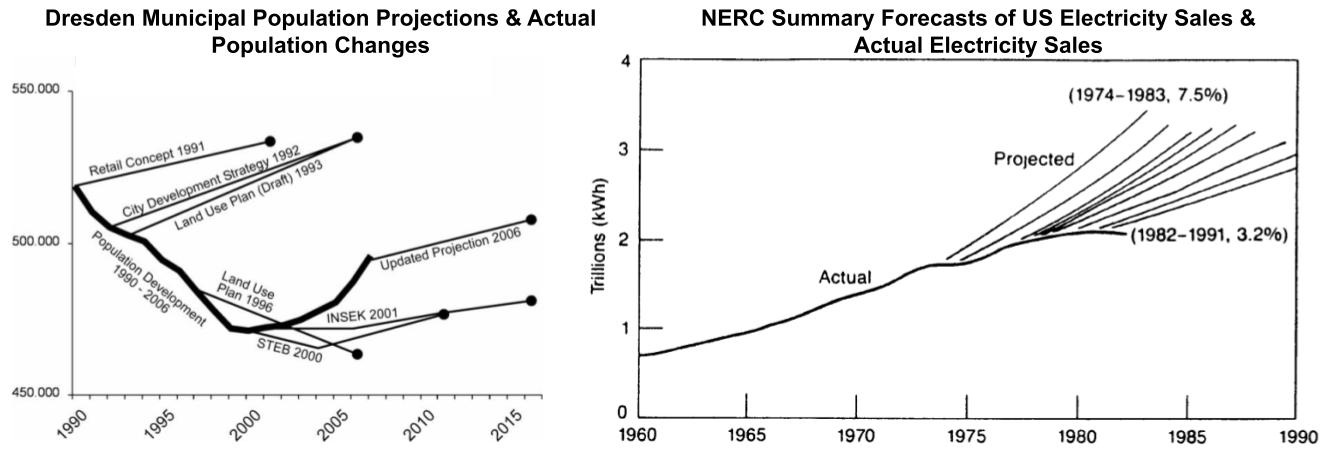
\includegraphics[scale=0.32]{Figures/chap2/projections.jpg}
	\caption[Projections compared to actual changes]{Left: Population changes in Dresden compared to various municipal projections. From \cite{wiechmannErrorsExpectedAligning2008}. Right: US National electricity sales compared with various NERC Summary Forecasts. From \cite{nelsonNERCFanRetrospective1985}}
	\label{fig:projections}
\end{figure}

One obvious response to this is, ``We just need better models." Miller, for example, argues that, despite the historical difficulties that integrated urban models have had, there is reason to be optimistic about the state of the art moving forward, particularly for integrating transportation and land-use models \cite{millerIntegratedUrbanModeling2018}. The potential and the weaknesses of this argument are addressed in Section \ref{sec:elitism} (and Section \ref{sec:se_critique} in particular). Another potential response is to avoid pursuing firm predictions and instead seek to gain provide some other benefit with the \ac{dss}. Bankes takes this approach, arguing that many of these problems can be avoided by clearly differentiating between \textit{consolidative models} that strive to be "a surrogate for the actual system" but are often out of reach, and \textit{exploratory models}, which seek to examine the implications of varying assumptions and hypotheses \cite{bankesExploratoryModelingPolicy1993}. Exploratory models are possible to construct more often than consolidative models, as they function in the absence of complete information, but this is only true if they are intentionally constructed as exploratory models with a specific aim.  To this end, Bankes defines three categories of purpose for an exploratory model: (1) data-driven, (2) question-driven, (3) model-driven. Most scenario planning, including the many of the historical examples that this work builds upon and the work described in this thesis are question-driven. For example, the 'What If?' tool from the late 1990s, explicitly "does not attempt to predict future conditions exactly. Instead it... can be used to determine \textit{what} would happen \textit{if} clearly defined policy choices are made and assumptions concerning the future prove to be correct" (emphasis in the original) \cite{klostermanWhatIfCollaborative1999}.

Wack agrees, writing that forecasting can be problematic as it constitutes ``someone else's understanding and judgment crystallized in a figure that then becomes a substitute for thinking." He then proposes scenario planning (particularly the exploratory variety) as an alternative, as it allows users to ``develop their own feel for the nature of the system, the forces at work within it, the uncertainties that underlies the alternative scenarios, and the concepts useful for interpreting key data" \cite{wackScenariosShootingRapids1985}. This raises the question if such alternative, non-predictive models and support tools are actually of real use to decision-makers. This is the essence of critique raised at the beginning of Section \ref{sec:critiques}. Due to the wide variety of \acp{dss} and planning practices, this is not a trivial question to answer.

To take scenario planning as a specific example, the evidence is decidedly mixed. Goodspeed's review of scenario planning use in urban planning and environmental research found only modest, ambiguous benefits (though use in industry management was more unambiguously positive) \cite{goodspeedScenarioPlanningCities2020}. He argued that many the applications in the review were poorly implemented, however. In particular he said that scenario planning was often misapplied to ``strategic planning" was anything but. ``A strategic plan might more closely resemble a project plan, with long lists of specific proposals and policies... many have relatively short time frames. Scenario planning may not make sense for these plans." His own study of impact of a scenario planning project in Lockhart, Texas, which sought to correct some of the flaws he perceived in many previous studies, confirmed that modest, but real positive changes are the result of scenario planning.

Others have pointed out that adopting a more participative process can improve outcomes. Zapata and Kaza provide evidence that scenario planning, particularly when incorporating diverse participants, can help planners cope with significant levels of uncertainty about the future (though they also note that few programs actually involve diverse participants) \cite{zapataRadicalUncertaintyScenario2015}. This extends beyond scenario planning with several sources confirming that higher levels of collaboration improves \ac{dss} functionality and usability \cite{goodspeedDeathLifeCollaborative2016, vonkSociotechnicalPSSDevelopment2010, brommelstroetPlanningSupportSystems2010, ulibarriCollaborativeModelDevelopment2018}. Notably, one of the early successes at combining remote observation imagery with socioeconomic data, the 1968 \ac{lunr}, elected to not use the military-developed land use classification schemes, but rather to interview future users about their needs and to use the results from these interviews to develop a classification system tailored to the application. Such benefits, particularly when contrasted with the failures of more technocratic approaches, demonstrate the differences between what philosopher and educator John Dewey ``a \textit{planned} society, which subordinates the present in pursuit of a rigid planned future, and a \textit{planning} society, which is intellectually preoccupied by the future but knows that only the present - and not the future can be controlled" (\cite{deweyHumanNatureConduct2007} as paraphrased by \cite{goodspeedScenarioPlanningCities2020}.

Even assuming that participative, model-based decision support has been conclusively been demonstrated to be helpful to decision-makers, there is still the question of whether such a project is the kind of science or engineering worthwhile for a doctoral thesis. I readily acknowledge and embrace the fact that this work is predominantly a piece of design science, which aims to ``design propositions, which inform specific practices, artifacts, or tools", rather than `conventional' science, which ``primarily aims to describe, explain, or predict the world but not to change it" \cite{goodspeedScenarioPlanningCities2020}. In fact, there are good reasons to avoid practicing ``conventional science" in these domains as treating society as a laboratory can lead to significant harms and a ``vivisectionist" mentality \cite{banandynuriModernMedicineIts1990}. This does mean there are certain limitations on this thesis. It cannot directly advance our fundamental understanding of mangroves, as an earth scientist might wish; our understanding of how cities change, as an urban planner might wish; or our ability to design satellites, as an aerospace engineer might wish. Nonetheless there is a certain and necessary purpose to be served by this piece of design science, as it seeks to help provide communities with the tools to decide their future.


%For the past couple of decades, there has been a recognition that \acp{dss} and \acp{pss} must include more than purely spatial analysis components \cite{geertmanPlanningSupportSystems2004}.



%Is not itself a means of planning and implementing projects. It is not a full life-cycle tool such as \ac{ppbs} \cite{hatryCriteriaEvaluationPlanning1972}

\section{\hlc[cyan]{Lessons \& Conclusion}} \label{sec:chap2-conc}

This chapter discussed a variety of fields with varying levels of connection, as well as some significant critiques of those fields and how they have been applied in recent centuries. The impetus of this chapter was the question:

\blockquote{ 1. What aspects of systems architecture (and systems engineering in general) are relevant and useful for approaching issues of sustainability in complex \acf{sets}? In particular, how can they be adapted using techniques from collaborative planning theory and other critical approaches to enable avoid the technocratic excesses of the past?}

Are we now prepared to answer it?

To start with, it is clear there are both major pull and push factors for bringing to bear systems engineering and other ways of making sense of data in complex systems on the issue of sustainability. Pull, in that our concepts of development and human wellness have expanded. They are no longer measured in short-term, purely individual economic of civil rights terms. We are considered with questions of equity, of ecosystem services, of community resilience. With this broadening has also come and increasing sense of urgency as we face various forms of resource depletion, environmental collapse, and climate change. The concept of sustainable development which seeks to capture both this broadness and urgency was discussed in Section \ref{sec:sustainable_development}. This section made it clear that there is a need for methods that can help with the planning and management of complex systems, particularly ones that involve humans, their technology, and the environment. 

The push factors are the increasing supply of such methods. Remote observation (Section \ref{sec:remote}) provides data that is new in kind, scale, and temporality. While it has a well developed history of monitoring environmental phenomena at the global scale, it has a much more limited use in local, human-centric applications and there is thus much potential there. Systems engineering (Section \ref{sec:se}) and \ac{gis} (Section \ref{sec:gis}) represent two approaches for corralling remote observation data along with that of many other sources for use in sustainable development. These two fields have been closely linked since their inception in the mid-20th century and both are based on the idea of using data and models to inform and support decision-making.

These fields are not unalloyed goods, however. Section \ref{sec:sdg_critique} explained how common definitions of sustainable development may have been watered down by entrenched powers and serve primarily to distract or co-opt more meaningful change. Section \ref{sec:technocracy} explained exactly what harms international development endeavors, be they ill-willed or good intentioned, can inflict. Sections \ref{sec:mapping_critique} and \ref{sec:se_critique} showed that \ac{gis} and systems engineering have often been key enablers of such harms.

So with these concerns in minds, just how can we ``avoid the technocratic excesses of the past?" Several recurrent lessons appear throughout this chapter. First is the importance of involving a wide set of stakeholders in a participative manner. The reasoning and history behind participative approaches is briefly summarized in Section \ref{sec:collaborative}. Often no single, objectives solution exists for a sustainable development problem and, even if it did, our data collection and analysis methods are insufficient to reach it. In absence of such a single solution, consider and selecting a course of action must be made by the community. Such a process helps too with acceptance and implementation of the decision. A wide set of stakeholders also commonly means both a wide concept of human wellness and one that is relevant to the community in questions. This means that the primary role of systems engineering and \ac{gis} in such situations is to support decisions rather than to make them, to help communities envision potential future scenarios rather than to dictate one to them. For this reason, decision support systems and scenario planning are presented in Section \ref{sec:scenario}.

What remains is the question of whether decision support is actually helpful and thus whether the topic is suitable for a doctoral thesis. Section \ref{sec:scenario_critique} addresses this. It reinforces the importance of participation in the development of useful \acp{dss} and argues that this thesis approaches it topic in a more responsible, and less technocratic manner. 

This chapter has thus supplied Research Deliverable 1a: ``A critical analysis of systems engineering, \ac{gis}, and the other fields relied upon in this work." The next chapter shall take the lessons learned here and apply them in the development of a framework for sustainable development work.